\documentclass[12pt]{article}
\usepackage[utf8]{inputenc}
\usepackage{amssymb}
\usepackage{wasysym}
\usepackage[a4paper, margin=2cm]{geometry}
\usepackage[dvipsnames]{xcolor}
\usepackage{graphicx}
\graphicspath{ {./images/} }
\usepackage{scrextend}

\usepackage{CJKutf8}
\newenvironment{Japanese}{%
  \CJKfamily{min}%
  \CJKtilde
  \CJKnospace}{}
%\begin{CJK}{UTF8}{}
%\begin{Japanese}

\title{\textbf{Learning Journal}}
\date{Date of last edit: \today}
\author{William Black 42920477}
\setlength{\parindent}{0pt}
\setlength{\parskip}{0.5em}
\setcounter{secnumdepth}{3}

\usepackage{hyperref}
\urlstyle{same}
\hypersetup{
    colorlinks=true,
    linkcolor=blue,
    filecolor=magenta,      
    urlcolor=cyan,
}

\begin{document}

\tableofcontents

\maketitle\section{11.08.19 - Proof of Concept: Scoping Exercise I}

Doing the Scoping Exercise first because the other task is recommended to be tackled in groups.

Time to find out how to use LaTeX.

\subsection{LaTeX}

First learning journal will be in Word since I don’t know how to use LaTeX yet.

Brian said to work in Rich Text and watch it come out perfectly on the right.

\subsubsection{\texorpdfstring{\underline{Error: Rich Text Mode}}{}}\label{error:er1}
\begin{itemize}
    \item Rich text mode in Overleaf does not come out perfectly on the right at all
    \item Sometimes code appears on the Rich Text version of the left
    \item The rich text options are extremely limited, it seems to just be bold, underline, bullet lists, and nothing else
\end{itemize}
\begin{itemize}
\renewcommand{\labelitemi}{}
    \item\underline{Solution:}
\renewcommand{\labelitemi}{$\bullet$}
    \item Don’t use Rich Text mode
\end{itemize}

Brian linked a \href{https://www.overleaf.com/learn/latex/Creating_a_document_in_LaTeX}{tutorial} for using Source mode.

Tutorial going smoothly.

Replacing parts of the tutorial result to reflect my Scoping Exercise.

Worked out using $\backslash$date\{$\backslash$today\} instead of typing out the date, magic!

\subsubsection{\texorpdfstring{\underline{Error: Bullet Lists}}{}}\label{error:er2}
\begin{itemize}
    \item Can’t work out how to make nested bullets.
\end{itemize}
\begin{itemize}
\renewcommand{\labelitemi}{}
\item \underline{Solution:}
\renewcommand{\labelitemi}{$\bullet$}
    \item \href{https://www.overleaf.com/learn/latex/Lists}{This tutorial} shows how to make nested bullets. Since I can, as a learning exercise, I want to combine bullets, bullets, and numbered lists.
\end{itemize}

I’m numbering the parts of my methodology, including the writing process and the bibliography creation. The pains and pain relievers can be bullets.

\href{https://www.overleaf.com/learn/latex/Lists}{The same tutorial} even shows how to change bullet list styles

\href{http://www.rpi.edu/dept/arc/training/latex/LaTeX_symbols.pdf}{This .pdf} is a list of different symbols I can use. 

\subsubsection{\texorpdfstring{\underline{Error: Using Packages}}{}}\label{error:er3}
\begin{itemize}
    \item Not working. Some of them work but most of them don’t.
\end{itemize}
\begin{itemize}
\renewcommand{\labelitemi}{}
\item \underline{Solution:}
\renewcommand{\labelitemi}{$\bullet$}
    \item Using \textbackslash usepackage\{\} with the package the symbol is from was surprisingly easy. I assumed I had to install something but just naming the package seems to work. 
    \item I wonder why they don’t just put something like “$\backslash$usepackage\{allpackages\}” at the beginning, and why not make that automatic?
\end{itemize}
    
Just realised I have to write gains and gain creators too, and I have the perfect bullet symbols for them. 

I kind of feel like some sort of genius hacker using LaTeX but my brain is starting to hurt, I’ve been fiddling around with the source editor for a few hours now.
There’s an option to collapse lists at the line numbers when you’re done writing them. It’s much easier to read. I’ve also realised I can separate the lines with single line breaks and nothing changes in the result, which also makes the code much more readable.

\subsubsection{\texorpdfstring{\underline{Error: Right Alignment}}{}}\label{error:er4}
\begin{itemize}
    \item Even with \href{https://www.overleaf.com/learn/latex/Text_alignment#Right-justified_text}{a tutorial} I can’t make a package work to allow me to make the date right-aligned and smaller.
\end{itemize}
\begin{itemize}
\renewcommand{\labelitemi}{}
\item \underline{Solution:}
\renewcommand{\labelitemi}{$\bullet$}
    \item 
\end{itemize}
    
Can’t figure out any solution to that problem so I’ll just leave it as is. I wanted to make the date a little less front-and-centre, but maybe the package isn’t working because it’s in the preamble.

But now it looks like I can change the format of the title, so that’s not the rule. \href{https://www.overleaf.com/learn/latex/Font_sizes,_families,_and_styles}{This tutorial} explains how to change font sizes, but rather than “12pt” etc it’s just larger or smaller than the size set at the beginning of the document.

Came across \href{https://www.overleaf.com/learn/latex/Paragraph_formatting#Reference_guide}{this tutorial} that tells me how to fix the automatic indenting. Looks nicer without it.


\subsubsection{\texorpdfstring{\underline{Error: Document Style}}{}}\label{error:er5}
\begin{itemize}
    \item The margins look kind of insane, they’re like two inches wide, and for some reason they’re even wider on only the second page. The first and third page look normal though.
\end{itemize}
\begin{itemize}
\renewcommand{\labelitemi}{}
\item \underline{Solution:}
\renewcommand{\labelitemi}{$\bullet$}
    \item After a lot of messing around with this tutorial to use the geometry package to make the margins more normal, I realised two-sided letter paper was still the document style set from when I was going through the set-up tutorial. I’ve made the paper A4 and one-sided.
\end{itemize}

While I don’t think these specific skills are necessarily going to be so handy in creating the ultimate Proof of Concept submission, learning how to search for things I don’t know how to do and familiarising myself with the logic of the program has been a difficult learning curve that I’m enjoying being on top of.

I’m finding it extremely confusing, how to submit the document. Someone else in class has submitted a .tex file, and now I reread the instructions, it does say specifically to upload either a .tex file or a word file on to cloudstor, not a .pdf. But there’s no button to download a .tex file, just a .pdf.

Okay an hour later I figure out you have to exit the program, and download a .zip of the file that contains the .tex file. 

Submitted the .tex file to Cloudstor, the .pdf to Turnitin.

Fingers crossed that next week’s task will take less than 6 hours now I’m more familiar with the program.

\subsection{Business Analysis: Pains and Gains}
The jobs involved in writing the project come down to methodology: Data collection; Contrastive linguistic comparison; Structural linguistic analysis; Writing the thesis. I wouldn't normally put a bibliography in there but since it's the one that keeps coming up as the example I can sense that this might end up being a relatively easy fallback for most students.

The pains and gains are tough to separate, obviously avoiding pain is a gain in itself.

There's no way for me to know whether any of these pain relievers/gain creators are possible to create programs for but this is apparently only to brainstorm, so we are pretending we live in a semi-magic world where small magics are possible, but not magic that's big enough to just do the entire thesis for me. Harry Potter rules.

\newpage
\section{12.08.19 - Data Carpentry: Spreadsheets}
Since yesterday’s task was so surprisingly complicated, I might see how I do with Data Carpentry solo and keep the tricky parts to ask my friends tomorrow.

\subsection{\textbf{\href{https://datacarpentry.org/spreadsheets-socialsci/00-intro/index.html}{\textbf{Introduction}}}}
\setlength{\parskip}{0.5em}


\color{Gray}\textbf{Questions}
\\What are basic principles for using spreadsheets for good data organization?

\textbf{Objectives}
\\Understand how to organize data so computers can make the best use of the data

\begin{itemize}
\renewcommand{\labelitemi}{}
\item \textbf{\underline{Exercise}}
\renewcommand{\labelitemi}{$\bullet$}
    \item How many people have used spreadsheets in their research?
    \item How many people have accidentally done something that made them frustrated or sad?
\end{itemize}\color{black}

I’ve used spreadsheets in research quite simply, just to find average values, or added values. A couple of times I tried to test for a null hypothesis, because I had just done Statistics 102 and I could still remember how to do it, but that was very complicated and I’m not 100\% confident doing it again now.

I don’t know if I’ve had that situation in the context of research… a few times a Windows update has interrupted me during an exam, which is scary, but I’ve just taken photos to prove I had a technical error. Definitely the worst one is when a Windows update restarts my computer and I’ve forgotten to save my Word file. It’s fine if you’ve saved it once, because AutoSave saves it for you, but if you haven’t saved and named it yet AutoSave doesn’t run.

\subsection{\textbf{\href{https://datacarpentry.org/spreadsheets-socialsci/01-format-data/index.html}{Formatting Data in Spreadsheets}}}

\color{Gray}\textbf{{Questions}}
\\What are some common challenges with formatting data in spreadsheets and how can we avoid them?

\textbf{{Objectives}}
\\Recognise and resolve common spreadsheet formatting problems.
\\Describe the importance of metadata.
\\Identify metadata that should be included with a dataset.
\color{black}

\vspace{1em}
\textbf{Data formatting} – always prioritise the computer understanding the data over you understanding it. You may need to format differently for different objectives.

\textbf{Keep track of analyses} – never clean/analyse/mess around with your original data, make a copy in a new tab/file and mess with that. Open the next tab to keep notes on what you did to end up with the new version, because you won’t remember in six months.

\textbf{Structuring data} – variables in columns, observations in rows, split all combined observations to simplest possible. When exporting cleaned data, use text-based format like comma-separated values (CSV)

\newpage
\color{gray}
\begin{itemize}
\renewcommand{\labelitemi}{}
\item \textbf{\underline{Exercise}}
\item We’re going to take a messy version of the SAFI data and describe how we would clean it up.
\end{itemize}
\begin{enumerate}
    \item Download the messy data.
    \item Open up the data in a spreadsheet program.
    \item Notice that there are two tabs. Two researchers conducted the interviews, one in Mozambique and the other in Tanzania. They both structured their data tables in a different way. Now, you’re the person in charge of this project and you want to be able to start analyzing the data.
    \item With the person next to you, identify what is wrong with this spreadsheet. Discuss the steps you would need to take to clean up the two tabs, and to put them all together in one spreadsheet.
\end{enumerate}
\color{black}

\begin{enumerate}
    \item Downloaded.
    \item Opened.
    \item Noticed tabs.
    \item There are too many things wrong with the data to just clean or fix. Some farmers would need to be re-interviewed or excluded from the sample if there’s no recording of the interview. Problems and solutions where possible listed below.
\end{enumerate}

\textbf{{Mozambique Data:}}
\begin{itemize}
\renewcommand{\labelitemi}{}
    \item \underline{Dwellings}
\renewcommand{\labelitemi}{$\bullet$}
    \item Some typos – mabati\_sloping instead of mabatisloping, errth instead of earth
    \item Most of the columns do not have spaces, presumably for algorithm reasons. “wall type”, “floor type”, “water use” should have their spaces replaced with underscores if that’s necessary.
    \item Farmer \#3 has -99 rooms in his dwelling, which is arguably too few.
    \item Farmer \#10 has five rooms in his dwelling including a barn. If the barn doesn’t count as a room, there should be a separate column for barns.
\renewcommand{\labelitemi}{}
    \item \underline{Livestock}
\renewcommand{\labelitemi}{$\bullet$}
    \item Farmer \#10 has no entry. If he has no livestock, it should say he has 0 so he is still included in the sample. Also check whether the missing entry really belongs to Farmer \#10, or if it is another farmer whose absence has moved the other farmers up a position in key\_id
    \item The number of livestock owned appears to be automatically generated from how many comma-separated animals are listed. This means that the number represents the number of TYPES of livestock owned, not the number of livestock. If number of livestock is needed, the farmers need to be re-interviewed and columns for each type of livestock should be made to record numbers of each type.
    \item Where “none” was entered, “1” type of livestock was recorded because the program assumed a none was a type of livestock. “none” entries should be replaced with “0”.
    \item Farmer \#10 has five rooms in his dwelling including a barn. If the barn doesn’t count as a room, there should be a separate column for barns. 
    \item For Farmers \#1 and \#5, “poultry” was counted as a type of livestock, where it was not for the other farmers.
    \item It is quite unlikely that Farmers \#2, \#4, \#5, and \#9 own cows but don’t look after them. Perhaps someone else has removed that responsibility from them but the researcher should check if that’s true.\renewcommand{\labelitemi}{}
    \item \underline{Plots}
\renewcommand{\labelitemi}{$\bullet$}
    \item “yes” and “no” are not consistent. Ideally, these values should be replaced with binary “1” = yes and “0” = no, or "yes" and "no".
    \item Farmers \#5 and \#10 have not had plots recorded. If they have no plots, “0” should be recorded.
    \item Where “none” was entered, “1” type of livestock was recorded because the program assumed a none was a type of livestock. “none” entries should be replaced with “0”.
    \item Farmer \#9 has -999 plots on his farm, which is arguably too few.
    \item Farmer \#2 only uses water during summer. If this affects the data, columns should be made for the seasons of Mozambique and Tanzania to record water usage in each season. If it does not affect data, then the most accurate answer is “yes”.
\end{itemize}

\textbf{{Tanzania Data:}}
\begin{itemize}
\renewcommand{\labelitemi}{}
    \item \underline{Dwellings}
\renewcommand{\labelitemi}{$\bullet$}
    \item If wall type, floor type, and look after cows categories should not have spaces in their cells, replace spaces with underscores.
    \item Farmer \#8 has 4 rooms including a cowshed. If a cowshed is not a room, there should be another column for cowsheds. underscores if that’s necessary.
\renewcommand{\labelitemi}{}
    \item \underline{Livestock}
\renewcommand{\labelitemi}{$\bullet$}
    \item Farmer \#10’s entry is missing. If he has no livestock then “0”s should be recorded. Also check whether the missing entry really belongs to Farmer \#10, or if it is another farmer whose absence has moved the other farmers up a position in key\_id.
    \item Many values are not recorded. If there are no livestock of that category, 0 should be recorded.
    \item Many of the totals do not equal the number of livestock recorded. Farmers need to be re-interviewed for correct numbers.
    \item Farmers \#4 and \#9 have cows and do not look after cows, which seems unusual. Researcher should check if that’s true.
    \item Farmer \#3 had a cow that died in April. The data should stipulate whether these values are for total owned during a particular period or a synchronic analysis. If the cow-owning was during the period, the Cows value should read “1”, and look\_after\_cows should read “yes”. If the number are only to reflect the situation at interview, look\_after\_cows should read “no”.
\end{itemize}

\textbf{Metadata} – The stipulations on your parameters (what counts as a room, is poultry a livestock, etc). This lesson discourages your from putting this information in the file but I can’t think of any reason putting it in a separate tab wouldn’t be a good idea. \color{teal}\small{- (16.08.19) The reason is for future compatibility. When saving in a universal format, tabs aren't saved. If you save in the Excel format, there may be compatibility issues with other programs, or other versions of Excel.}

\color{gray}
\begin{itemize}
\renewcommand{\labelitemi}{}
\item \textbf{\underline{Exercise}}
    \item Download a clean version of this dataset and open the file with your spreadsheet program. This data has many more variables that were not included in the messy spreadsheet and is formatted according to tidy data principles.
    \item Discuss this data with a partner and make a list of some of the types of metadata that should be recorded about this dataset. It may be helpful to start by asking yourself, “What is not immediately obvious to me about this data? What questions would I need to know the answers to in order to analyze and interpret this data?”
\end{itemize}

\color{black}
\begin{itemize}
\renewcommand{\labelitemi}{}
    \item The variables need to be defined for a human to read this. Years\_liv might be years at the address, years that the farm has been functioning, years in the village, etc. Months\_lack\_food might be over the past calendar year, the last 12 months, it might be a lack of human food, livestock food, or lack of food produced by the farm
    \vspace{0.5em}
    \newline Affect\_conflicts appears to be a multiple-choice answer, so we need all the options that were available to interviewees.
    \vspace{0.5em}
    \newline Some definitions need to be made like, what counts as a “room” in the dwelling.
\end{itemize}

\newpage\section{14.08.19 – Data Carpentry: Spreadsheets}

\subsection{\textbf{\href{https://datacarpentry.org/spreadsheets-socialsci/02-common-mistakes/index.html}{\textbf{Formatting Problems}}}}

\underline{Common Spreadsheet Errors}
\begin{itemize}
    \item Using multiple tables
    \begin{itemize}
        \item Confuses the computer, who assumes that Column D will be the same variable for any Row.
    \end{itemize}
    \item Using multiple tabs for like data
    \begin{itemize}
        \item Any information put in separate tabs is not able to interact with earlier tabs, so it wouldn’t be good for things like new measurements of same variables
        \item Under the View menu there’s an option to freeze top row or left column so you can still see them when you’re deep in the spreadsheet
    \end{itemize}
    \item Not filling in zeros
    \begin{itemize}
        \item If you don’t fill in zeros, you don’t know if there are none or if you just haven’t measured the variable yet
    \end{itemize}
    \item Using problematic null values
    \begin{itemize}
        \item Apparently some people put -999 for null values. It’s obvious why that’s not a good idea
    \end{itemize}
    \item Using formatting to convey information
    \begin{itemize}
        \item Don’t add a comment to a cell, the computer can’t read it. If the comment is important to the data, it’s a new variable and needs its own column.
    \end{itemize}
    \item Using formatting to make the data sheet look pretty
    \begin{itemize}
        \item Don’t merge cells, stats software can’t read it
    \end{itemize}
    \item Placing comments or units in cells
    \begin{itemize}
        \item Software can’t read it
    \end{itemize}
    \item Entering more than one piece of information in a cell
    \begin{itemize}
        \item Every aspect of information that’s important is its own variable with its own column. If it’s not important it doesn’t need to be in the cell
    \end{itemize}
    \item Using problematic field names
    \begin{itemize}
        \item No spaces because some software uses spaces as delimiters. No special characters. Numerals are allowed but ideally avoided so they don’t get caught up in your observations. 
    \end{itemize}
    \item Using special characters in data
    \begin{itemize}
        \item To avoid cutting off elements, treat the spreadsheet like a web form that can only contain plain unformatted alphanumerical characters
    \end{itemize}
\end{itemize}


\underline{Problematic Data Produced by my Discipline}

\vspace{1em}
I’m an interdisciplinary student and have three disciplines to choose from, but I’ll go with Media \& Communication since this semester is quite focused on that framework in my process.

This isn’t exactly a “bad spreadsheet”, but this is an example of poor design with missing variables that’s bothered me for a few years now – why on earth would movies be ranked or have their success judged based on gross earnings? 

Let’s allow for the argument that we judge merit based on earnings as quantifiable numbers rather than based on unquantifiable “inspiration” or “enjoyment” etc.
 
Here is a spreadsheet of the top-earning films of 2018. 

\vspace{1cm}
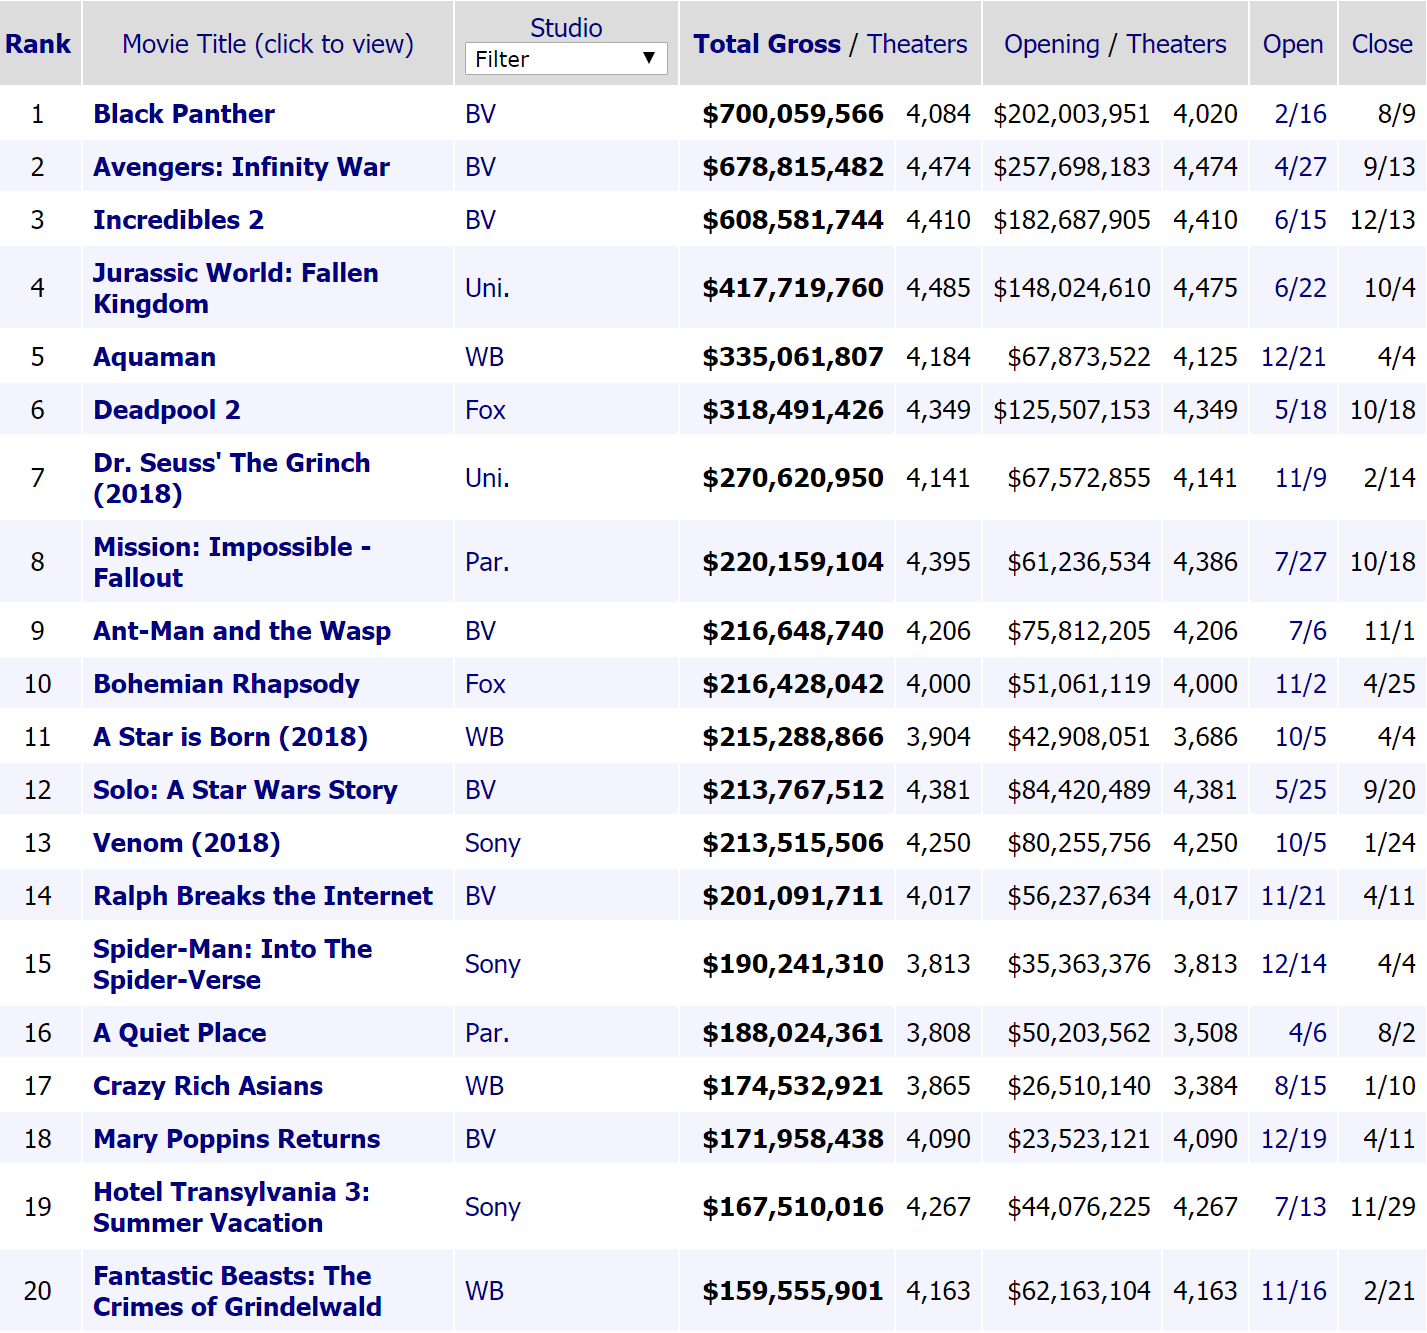
\includegraphics[width=\textwidth]{imgtopfilms.png}

\vspace{1em}
\newpage
\textbf{Problems:}
\begin{enumerate}
    \item \underline{The films were released at different numbers of cinemas}
    \vspace{0.5em}
    \\For example, A Quiet Place earnt less than Jurassic World, but was available at 3808 cinemas to Jurassic World’s 4485 cinemas.
    \item \underline{The films were released at different cinemas}
    \vspace{0.5em}
    \\Each cinema sets its own ticket price, and has different deals for cheap Tuesdays, discounts, promotional prices with nearby restaurants, etc. The amount grossed does not give any indication of how many audience members saw the film or the success of the film, because there are no numbers on how many cents of each ticket price is taken by the cinema.
    \item \underline{What year they opened and closed}
    \vspace{0.5em}
    \\This is more a problem with the design of the spreadsheet itself than the design of the project, but the dates for opening and closing are ambiguous. I might guess, looking at the numbers, that the dates are formatted mm/dd, but there is no year on either to show how long they were open for. Even though this list is for 2018, there’s no indication whether it is the opening dates or closing dates that occur in 2018. I might guess opening, just based on my background knowledge of the titles in the list, but then it doesn’t necessarily follow that the closing year is 2019, many films may be in cinemas for over a year. Rocky Horror Picture Show is still being played at cinemas since 1975.
    \item \underline{They were open for different lengths of time}
    \vspace{0.5em}
    \\The Grinch did not perform as well as Incredibles 2, but it had literally half the time within which to earn that money. If the data divided the gross by average grossed per day, this would be a very different spreadsheet
    \item \underline{Biggest problem: They have different production budgets}
    \vspace{0.5em}
    \\If we’re happy to commit to financial earnings being our metric for success, amount grossed is not a logical approach. Financial success should tell you what production companies/directors/actors are the safest financial investments for investing distribution companies, portfolios managers, etc., but this does nothing to show what kind of return these titles made on their investments, only how much money was received. 
    \vspace{0.5em}
    \\For a film like Jurassic Park, ranked \#4 due to grossing ~\$418 million, the production budget was ~\$170 million, meaning that the amount earnt by the movie was approximately 245\% of its investment. 
    \vspace{0.5em}
    \\A Quiet Place, for comparison, ranked at \#16 for grossing \$188 million, but had a meagre production budget of \$17 million, meaning that the film earnt 1,106\% of its investment.
    \vspace{0.5em}
    \\For Fantastic Beasts: The Crimes of Grindelwald, the production was ~\$200 million, meaning that the film actually LOST \$40 million, and yet is ranked \#20 on the most successful films of 2018. 
\end{enumerate}

\newpage\section{16.08.19 - Transferring the Learning Journal to Overleaf}

\subsection{LaTeX}
\subsubsection{\texorpdfstring{\underline{Error: Paragraph Spacing}}{}}\label{error:er6}
\begin{addmargin}[1cm]{0cm}
Struggling to work out how to start a new paragraph rather than new line. 

\underline{Solution:}

New line can be made with just two backslashes without using $\backslash$newline.

New paragraph can be made with $\backslash$par, but isn't a proper paragraph break.

Two enter-breaks can also be used for a paragraph break.

I found an option to $\backslash$parskip\{1em\}. It's a toggle that can be used in the preamble and set through the document.

\textcolor{teal}{- (19.08.19) I saw someone on Slack suggest using $\backslash$vspace\{1em\} for one-off instances of stretching, which is exactly what I was looking for.}


\end{addmargin}

What's an em? \color{teal}{\small{- (19.08.19) An "em" is the space an M takes in the current font. That's quite handy because it's a measurement that changes with the font size.}}

\color{black}
My word document had a lot of hyperlinks, 
\href{https://www.overleaf.com/learn/latex/Hyperlinks}{here} is a tutorial on making hyperlinks. Now I can insert all the hyperlinks I had in the original document

\subsubsection{\texorpdfstring{\underline{Error: Special Characters}}{}}\label{error:er7}
\begin{addmargin}[1cm]{0cm}
I'm having a problem with special characters in Overleaf such as \% and \$ and $\backslash$. They have functions in Overleaf so I can't use them as text characters without them performing their functions.

\underline{Solution:}

I worked out you can use a backslash before most of the special characters to stop them from getting formatted in the main document (thanks, Reddit addiction), but that doesn't work on backslashes. I also can't think of a good way to google that, "how to use backslashes in Overleaf" is only getting me how to use them as a function, of course.
\\\textcolor{teal}{- (19.08.19) Couldn't stay long enough after class to get my questions answered, but found an answer on a forum to insert the $symbol$ of a backslash as \texttt{"\$$\backslash$backslash\$"}.}
\end{addmargin}

\section{19.08.19 - Still transferring the Learning Journal to Overleaf}
\subsection{LaTeX}

\texttt{$\backslash$texttt} makes fonts monospace, I'll keep that going from now on.

I'm starting to get the hang of how to run Overleaf now. You really just google everything you want to do and there's always a tutorial for it somewhere. 

\subsubsection{\texorpdfstring{\underline{Error: Image Insertion}}{}}\label{error:er8}
\begin{addmargin}[1cm]{0cm}
I'm a bit confused about how to get an image in - I used one for explaining the bad data from my discipline. In Word I just clipped it with the clipping tool and ctrl+Ved to Word. The tutorial seems to have 5 different ways that I understand equally poorly.

\underline{Solution:}

I had to add the package to the preamble. The directory is the directory on Overleaf, not my directory.

You can set the width of the image to equal the text width with 
\\\texttt{$\backslash$includegraphics[width=$\backslash$textwidth]\{imagefilename\}}
\end{addmargin}

\vspace{0.5em}
Wow I didn't realise I had a directory, actually I've put this learning journal in a folder called "Scoping Exercise".

Frankly, I'd like to keep these together so I can easily find codes I used elsewhere. I'll just rename the folder to be all-purpose. "William-Black-Exercises" to avoid spaces.

I also had a look at indenting entire paragraphs before, I wonder if I just forgot a package in the preamble like for the graphics.

Yes I did.

\subsubsection{\texorpdfstring{\underline{Error: Margins}}{}}\label{error:er9}
\begin{addmargin}[1cm]{0cm}
I want to indent the whole paragraph, not just the first line, because it's quite difficult to read different section that lie in the same space like this.

\underline{Solution:}

I had to add the scrextend package to the preamble. Now I can use $\backslash$begin\{addmargin\}[1cm]\{0cm\} to make left margin 1cm and right margin 0cm, and $\backslash$end\{addmargin\} to indent whole paragraphs.

\end{addmargin}

This is getting a lot easier. I've only spent 2:30hrs on the journal today and I transferred the entire thing including this entry I'm making now.

To be honest, I'm really unaware of any situation where this would be faster or easier than a regular word processor but I'm trusting I'll eventually find one!

\newpage\section{19.08.19 - Data Carpentry: Spreadsheets}

\subsection{\href{https://datacarpentry.org/spreadsheets-socialsci/03-dates-as-data/index.html}{\textbf{Dates as Data}}}

\color{gray}
\underline{Questions}

What are good approaches for handling dates in spreadsheets?

\underline{Objectives}

Recognise problematic or suspicious date formats.
\\Use formulas to separate dates into their component values (e.g. Month, Day, Year)
\color{black}

\vspace{1em}
\textbf{Date formats in spreadsheets} - It is $not$ best practice to store dates in one column, ideally you have a day, month, and year column.

\textbf{Dates stored as integers} - Excel stores dates as days from 31 Dec 1899, which can be useful if you need to average durations or study the dates as integers.

\textbf{Regional date formatting} - While there is an option to make date format suit your region, you'll forget to set it or US researchers will forget to adjust it or will try to adjust it when you already did.

\color{gray}
\vspace{1em}
\underline{Exercise:}
\begin{enumerate}
    \item Download and open the dates.xlsx file. This file contains a subset of the data from the SAFI interviews, including the dates on which the interviews were conducted.
    \newline Choose the tab of the spreadsheet that corresponds to the way you format dates in your location (either day first DD\_MM\_YEAR, or month first MM\_DD\_YEAR).
    \item Extract the components of the date to new columns. For this we can use the built in Excel functions:
    \newline =MONTH(), =DAY(), =YEAR()
    \newline Apply each of these formulas to its entire column. Make sure the new column is formatted as a number and not as a date.
    \newline We now have each component of our date isolated in it’s own column. This will allow us to group our data with respect to month, year, or day of month for our analyses and will also prevent problems when passing data between different versions of spreadsheet software (as for example when sharing data with collaborators in different countries).
    \item Using the same spreadsheet, add another data point in the interview\_date column by typing either 11/17 (if your location uses MM/DD formatting) or 17/11 (if your location uses DD/MM formatting). The Day, Month, and Year columns should populate for this new data point. What year is shown in the Year column?
\end{enumerate}
\color{black}
\begin{enumerate}
    \item No problem.
    \item Took me a sec on google to remember how to do this. I'm rusty.
    \item 2019. If you don't put a year, it assumes you want the current one. This means if I am working with data from another unknown year I will need the 3-column system to have a null value for the year.
\end{enumerate}

\textbf{Historical data} - dates from before 31 Dec 1899 are not parsed by Excel. 

\newpage
\subsection{\href{https://datacarpentry.org/spreadsheets-socialsci/04-quality-assurance/index.html}{\textbf{Quality Assurance}}}

\color{gray}
\underline{Question:}

How can we carry out basic quality assurance in spreadsheets?

\underline{Objective:}

Apply quality assurance techniques to limit incorrect data entry.
\color{black}

\vspace{1em}
\textbf{Validating data on input} - Data is restricted to numeric range or controlled vocabulary.

\textbf{Restricting data to a numeric range} - Select the whole column. Data $\rightarrow$ Data Tools $\rightarrow$ Data Validation. You can set it to only allow sensible numbers.

\vspace{1em}
\color{gray}\begin{addmargin}[1cm]{0cm}
\underline{Exercise:}

Apply a new data validation rule to one of the other numeric columns in this data table. Discuss with the person sitting next to you what a reasonable rule would be for the column you’ve selected. Be sure to create an informative input message.


\color{black}
I'll assume the years\_farm variable is how many years the interviewee has personally been running their farm. Acceptable answers would be 1-100, as less than a full year would be too short for the research aims, and over 100 would be too old to be running a farm, or a confused interviewer who thinks the question is regarding the farm's existence. I'd only take whole integers, because interviewees may struggle to remember the date they took command of their farm, and then data would vary in specificity.

I made my input message title "Whole years interviewee has run farm (1-100)" which displays when hovering over the cell.
\end{addmargin}

\vspace{1em}
\color{black}
\textbf{Restricting data to entries from a list} - Select variable column $\rightarrow$ Data $\rightarrow$ Data Tools $\rightarrow$ Data Validation again. Allow: List will give you a Source box, where you can list the possible answers separated by commas.

\vspace{1em}
\color{gray}\begin{addmargin}[1cm]{0cm}
\underline{Exercise:}

Apply a new data validation rule to one of the other categorical columns in this data table. Discuss with the person sitting next to you what a reasonable rule would be for the column you’ve selected. Be sure to create an informative input message.

\color{black}
The floor\_type variable has limited possible answers, so I could list "cement, earth". Personally, I don't know enough about floors or rooves or walls to know what options are possible. The input message should list the possibilities.
\end{addmargin}

\color{black}
\vspace{1em}
\section{20.08.19 - Data Carpentry: Spreadsheets}

\subsection{\href{https://datacarpentry.org/spreadsheets-socialsci/05-exporting-data/index.html}{\textbf{Exporting Data}}}

\color{gray}
\underline{Question:}

How can we export data from spreadsheets in a way that is useful for downstream applications?

\underline{Objective:}

Export data from a spreadsheet to a CSV file.

\color{black}

\textbf{Storing data} - Do not save as the default formats .xls or .xlsx, due to compatibility issues. R packages can often read them but may have issues with newer versions. Even Excel's own rules can change between versions. Save as TSV (Tab-Separated Values) or CSV, so you can even open it in Notepad, but it still works perfectly in Excel. Can't save multiple tabs. Save as $\rightarrow$ .csv. (If the data has commas, remove them or enclose field with double quotes.)

\section{20.08.19 - Proof of Concept: Scoping Exercise II}

\subsection{LaTeX}
\vspace{1em}
I'll start the document by copying the code from Scoping Exercise I, so I have all the same formatting, date, author, etc.

\subsubsection{\texorpdfstring{\underline{Error: Automatic Dating}}{}}\label{error:er10}
\begin{itemize}
    \item Just realised the \texttt{$\backslash$date\{$\backslash$today\}} trick is going to be the wrong date once the date changes.
\end{itemize}
\begin{itemize}
\renewcommand{\labelitemi}{}
\item \underline{Solution:}
\renewcommand{\labelitemi}{$\bullet$}
    \item When dating work on a continuing document, the date should be written out unless the date is something that will change, such as date last edited.
\end{itemize}

Whoops! I'll keep it at the top of this Learning Journal because then you can see the date of last edit.

\section{23.08.19 - Proof of Concept: Scoping Exercise II}
\subsection{Understanding Scoping Exercise II}
Feedback on Scoping Exercise I: "It seems like your ideas fall into two broad categories, firstly the collection, transcription, translation and analysis of Disney song lyrics and, secondly, writing and referencing your actual thesis. Either of these would be really interesting and useful to pursue."

I agree that the collection, transcription, translation and (comparative) analysis of Disney song lyrics is essentially the mission of the research, but can a computer do that?
 
After staring at these instructions for a couple of hours, here are all the things I don't understand:
\begin{itemize}
    \item Is Scoping Exercise II supposed to find one specific problem to solve or is "collection, transcription, translation, and comparative analysis" a problem I can solve if I can define the boundaries well enough?
    \item The general feedback from the marker: "Part of the scoping process, which was not so well done in the assignment, is the part where students narrow their focus in to one individual idea or group of ideas, ie the pain / gain which you are going to work on this semester as your Proof of Concept / Technology Deployment." 
    
    We were not told to do this in the instructions for Scoping Exercise I, and we \textit{are} told to do this for Scoping Exercise II. If this was the aim of Scoping Exercise I, then what is the required elaboration in Scoping Exercise II?
    \item More feedback: "A number of you jumped straight into finding solutions for your pains / gains, without fully identifying the boundaries of what you are attempting to do. Defining what is both inside and, just as importantly, outside the scope of your project is a key step that will save you both time and frustration."
    
    What is a pain reliever or a gain creator if not a solution to a pain or gain? Identifying the boundaries of what I'm attempting to do is absolutely something that can't be skipped, but the exercise was said to be to "brainstorm" what barriers occur in my research and what it would look like to remove them.
    \item How wishful am I supposed to be with a tool that assists me with research? Since I've no idea what a computer can or can't help with, I don't know how to create a realistic tool, and it seems like there should be some boundaries on how wishful my tool should be.
    
    I suggested that my tool could collect, transcribe, translate and analyse the comparison of the translations, which Brian said looked "great". I assume a computer can't do that though, so what's to stop me aiming for a tool that automatically writes the thesis for me?
    
    \item I cannot understand the Rubric for this task at all. It seems like the Rubric is designed to cover the entire process up to submission at the end of semester, but there is no indication which parts cover which individual tasks.
    
    \item I have found this in the Week 3 Summary: "Scoping Exercise Deadline: Firstly, the initial scoping exercise is due on Sunday 18 August at 11.59pm. This task will be assessed and is the first milestone of your Proof of Concept or Technology Deployment (PoC/TD). The scoping exercise should be submitted via Turnitin. The rubric for the scoping exercise is the first *three* lines of this document [the rubric] and further information on how to approach this assignment and what is required can be found in the 'Proof of Concept Scoping 101' section of the week 2 lecture slides."
    
    As far as I was aware, this task was due on Friday, and I had already submitted it. The explanation of what part of the rubric is used to mark us has to be given before we start the task, not after we submit it. Even giving this explanation on Friday and giving an extension until Sunday is not adequate - I had no notice and I was working 6:00-19:00 that weekend!
    
    What part of the rubric is for this task?
    
    \item This task is not being graded, so does it have a rubric? If not, should I just interpret the instructions in a way that makes sense?
    
    \item Found this message on Slack: 
    \begin{itemize}
    \renewcommand{\labelitemii}{}
        \item \texttt{Brian 4:39 PM}
        \item Important trap. At the end of the unit, during the final submission for the proof of concept, for the HD "Demonstration of Capability" I wrote: "Proof of Concept achieves goals articulated in the scoping document using tools and techniques tested in elaboration. PoC runs without errors and credibly demonstrates a route for implementation in planned research. PoC matches the product described in the OSP exactly."
        \\So while this is not being graded, it's important to take it seriously
    \end{itemize}
    So the tools and techniques I... "test" in Scoping Exercise II must be used to achieve a goal I specified in Scoping Exercise I? That's just a guess, because:
    \begin{itemize}
        \item Nothing has been labeled as "scoping document" or "elaboration". What do these terms mean?
        \item There is nothing in the instructions for Scoping Exercise II that instructs me to test tools or techniques, only to "decompose" a problem, "recognise patterns" in the data, and to "design an algorithm". If I am supposed to test tools and techniques, that needs to be in the instructions.
        \item We have no idea what the OSP is yet. All we have from the unit guide is "You will write an 'Original Software Publication' (OSP) article appropriate for a software journal detailing your analytic pipeline using the TeX SoftwareX article template provided."
% Original Software Publication is a type of journal article.        
        ... Write an article? Which is it, an article or a software publication? 
        - What's an analytic pipeline? 
    \end{itemize}
    \item The \href{https://unitguides.mq.edu.au/unit_offerings/95891/unit_guide#assessment_task_257486}{unit guide} for this course only specifies four gradeable tasks: three in Weeks 12 and 13, and one that is marked weekly (the learning journal). I'm pretty sure the university does not allow changes to this without having a new unit guide approved, and we are not allowed to be graded on other assessments outside those parameters.
    \item The instructions for Scoping Exercise II are in three steps:
    \begin{enumerate}
        \item \textbf{Decomposition:} First (and most important), decompose the activities that involve ‘pains’, opportunities for ‘gains’, and any solutions you proposed into small parts and/or discrete steps.
        \begin{itemize}
            \item The painful \textit{activities} and gainful \textit{opportunities} are broken down into small steps? How do you do that? 
            \begin{itemize}
                \item Pain: Translating a Japanese lyric set 
                \\Step 1: Get the lyrics from online somewhere 
                \\Step 2: Translate the first line
                \\Step 3: If unknown kanji appears, look it up on jisho.org
                \\Step 4: If line does not appear to make sense, check for other meanings on weblio.jp
                \\Step 5: If line still does not appear to make sense, google the phrase in quotes to see other contexts in which it's used if it's a common phrase, or sometimes if it's an uncommon phrase a native Japanese person will be asking what the phrase means online.
                \\Step 6: Translate next line
                \\Repeat Steps 3-6.
                \vspace{0.5em}
                \item Gain: It would be great if lyrics were already checked for accuracy
                \\Step 1: That would be great.
                \vspace{0.5em}
                \item Gain: It would be great if a program could automatically fill an Excel sheet formatted to equal bar length so I could assign fidelity values to line pairs easily.
                \\Step 1: The program would retrieve the lyrics
                \\Step 2: It would format the lyrics to equal bar length
                \\Step 3: It would fill an Excel sheet with Spanish, English, and Japanese variable columns for each line of song in rows.
                \\Step 4: That would be great.
            \end{itemize}
            \item Also any \textit{solutions} I proposed in Scoping Exercise I are broken down in to small steps
            \begin{itemize}
                \item Firstly, the marker gave us feedback that we were NOT supposed to come up with solutions in Scoping Exercise I
                \item How do you break down a solution that doesn't exist/doesn't exist yet into smaller steps?
                \vspace{0.5em}
                \item Gain creator: A program that could listen to music and autogenerate the lyrics in any language.
                \\Step 1: Learn how to make program
                \\Step 2: Use newfound skill to make the program
                \\Step 3: Run the program
                \vspace{0.5em}
                \item Obviously breaking this down doesn't make sense because I don't know what steps are involved apart from "find out what steps are involved". And I don't know if this is possible with current technology, so I also don't want to be penalised later when I can't fulfil my stated goal.
                \end{itemize}
        \end{itemize}
        \item \textbf{Pattern Recognition:} Next (if possible), identify patterns in the problems you are trying to solve or the solutions you are proposing.
        \begin{itemize}
            \item If possible? So this part is not a requirement? 
            \item Earlier in the same instructions, Pattern Recognition was about recognising patterns in data, not in problems or solutions. Is it data, or problems and solutions?
            \item The real pattern for all of them is that I don't know how to solve the problems, if they can be solved, or what steps one might take to solve them.
        \end{itemize}
        \item \textbf{Algorithm Design:} Finally, revise the solutions you developed during Business Analysis to produce a step-by-step guide describing what you want to accomplish.
        \begin{itemize}
            \item First of all, the marker gave us feedback on Slack that we were NOT supposed to come up with solutions in Scoping Exercise I.
            \item What is Business Analysis? - I asked Brian on Slack and he confirmed Business Analysis is another name for Scoping Exercise I.
            \item How can a step-by-step guide that "describes a goal" be produced? I guess maybe it means a step-by-step guide to \textit{achieving} the goal, but that doesn't make sense either because how can I magically know how to achieve a goal I'm not even sure is possible to achieve? If I knew what the solution to the pain point was, obviously it wouldn't be a pain point because I would just carry out that solution. 
        \end{itemize}
    \end{enumerate}
    \item Although it doesn't say in the instructions (it should REALLY say this in the instructions!!), more information from Slack suggests we are supposed to focus on ONE specific, useful, achievable proof of concept/tech demonstration.
    \begin{itemize}
        \item How can a proof or a demonstration be specific, useful, and achievable? I think I STILL don't know what a proof of concept or a tech demonstration is.
        \item Does this mean the PoC and the TD are the same thing? Because they are two separate assignments in this course
        \item Brian elaborates, "We're taking all of the possible problems you could solve and finding one that is worthy of solving in the time available." How am I to know what problem is worthy? How am I to know what problem can be solved within 10 weeks? How am I to know what problem can be solved? Am I supposed to guess? If I guess wrong, my marks for the assessment suffer because I didn't use the techniques and tools that I was supposed to "test" in this exercise. - Whatever "test" might mean in this context.
    \end{itemize}
    \item Am I the one that's insane here? I know from 4 years of university study that usually when I'm confused, everyone else is just as confused as me but less likely to articulate it and be specific about it than I am. But still. This is a LOT of people who would be just guessing what to do and are satisfied with whatever result comes. Surely someone else is concerned about this??
\end{itemize}

\newpage\section{26.08.19 - Proof of Concept: Scoping Exercise II}
\subsection{Computational Analysis: Decomposition, Patterns, Algorithm Design}
Now I've had my questions cleared up by Shawn and Brian I can start the task. 

\textbf{Decomposition}

I should break down the pains/gains I listed in Scoping Exercise I into a step-by-step process of what I currently have to do for each pain manually, into as many steps as would be required for a researcher from a different discipline to be able to follow. 

Hard to know exactly how far to decompose this, because for something like data acquisition, for mine I would certainly need to a bunch of things to decide how to SELECT what data to acquire. 

I'll try to cover everything I can think of, it won't matter if it's overkill because Pattern Recognition stage will work out what's useful.

\subsubsection{\texorpdfstring{\underline{Error: Displaying Japanese Characters}}{}}\label{error:er11}
\begin{itemize}
    \item None of the Japanese characters are displaying when I compile the code.
    \item A lot of the suggestions I'm finding online for typing in Japanese are suggesting packages that don't work, perhaps because they are designed for things called "XeTeX" or "pTeX" or "LuaLaTeX", which I'm guessing might be a different format to LaTeX
\end{itemize}
\begin{itemize}
\renewcommand{\labelitemi}{}
\item \underline{Solution:}
\renewcommand{\labelitemi}{$\bullet$}
    \item I finally found a \href{https://tex.stackexchange.com/questions/68333/how-to-put-japanese-kanji-characters-into-an-english-document}{forum support question} that specifically asks how to insert Japanese characters into English documents.
    \item Although the answer at this link is incorrectly formatted, the package CJKutf8 does work, if you begin and end \texttt{\{CJK\}\{UTF8\}} and \texttt{\{Japanese\}} around the begin and end lines of \texttt{\{document\}}.
\end{itemize}

\textbf{Pattern Recognition}

Although I expected to need to pick one or two favourites out of perhaps 6 possible robots, the decomposition process has resulted in two neat categories: Getting canon lyrics automatically populated to a spreadsheet ready for me to analyse; and helping me write and reference my research the way I want.

I remember Shawn said the first process may not be as difficult as I think, but it's awfully niche-use. If I could really make a framework that would help me stay on my writing, I could use that for every thesis I ever write, which would be amazing. I suppose PoCs for citations are kind of the "fallback" PoC project for this class, but I'm really tempted by this one because it would also \textit{organise} me which is my main barrier of ADHD to overcome. Doing it by hand as I do now is extremely effective but it does take a lot of extra time.

\textbf{Algorithm Design}

I didn't realise until typing this out how great a writing frame would be, I really want that to exist already so I can use it for my 6000 word essay this semester. 

I wonder how difficult it would be to make something visual like that? I'm an ex-graphic designer, I could make it look cute to use and everything. 

I also wonder how possible it would be to make something that interacts with... Word, say. I suppose you ought to avoid making something that is at the mercy of Microsoft's current version of Word, but I'm not about to be capable of making my own word processor either.

\newpage
\section{27.08.19 - Data Carpentry: Unix Shell}

\subsection{\href{http://swcarpentry.github.io/shell-novice/01-intro/index.html}{\textbf{Introducing the Shell}}}

\color{gray}
\underline{Questions}

What is a command shell and why would I use one?

\underline{Objectives}

Explain how the shell relates to the keyboard, the screen, the operating system, and users’ programs.

Explain when and why command-line interfaces should be used instead of graphical interfaces.
\color{black}

\vspace{1em}
\textbf{Background}

Computers can
\begin{enumerate}
    \item Run programs
    \item Store data
    \item Communicate with each other
    \item Interact with us
    \begin{itemize}
        \item Usually through a GUI (Graphical User Interface). 
        \\Pros: Intuitive
        \\Cons: Giving thousands of instructions takes hours
        \item Or through a CLI (Command-Line Interface)
        \\Pros: An instruction can be repeated or repeated with modifications thousands of times within minutes
        \\Cons: Not intuitive
        \\Interaction happens through the REPL interface (Read-Evaluate-Print-Loop interface). When you type a command and press enter, it \textit{reads} command, \textit{evaluates}/executes command, \textit{prints} output of command, \textit{loops} back to square one to await your next command.
    \end{itemize}
\end{enumerate}

\subsubsection{\texorpdfstring{\underline{Error: GUI/CLI Confusion}}{}}\label{error:er12}
\begin{itemize}
    \item Although I just wrote those notes, I still don't really know what a GUI or CLI are. Is it the difference between a command prompt screen and.. an algorithm program?
\end{itemize}
\begin{itemize}
\renewcommand{\labelitemi}{}
\item \underline{Solution:}
\renewcommand{\labelitemi}{$\bullet$}
    \item \href{https://study.com/academy/lesson/what-is-a-graphical-user-interface-gui-definition-components-examples.html}{This page} explains it a bit more simply: the GUI (pronounced Gooey! Cute!) is like regular Windows Explorer or any of the others, so you interact with the mouse and click on the stuff. Yes, very intuitive in comparison. The CLI is like Unix or whatever interface I used to use to get into Number Munchers when I was a wee kitten.
\end{itemize}

\textbf{The Shell} runs other programs rather than doing its own thinking. The most popular shell is called Bash. It is \textit{probably} the one I'm using for this exercise. It uses a dollar sign for a prompt so I think we're in.

First command to try is \$ 1s.

\subsubsection{\texorpdfstring{\underline{Error: Shell Command Not Found}}{}}\label{error:er13}
\begin{itemize}
    \item Typed \texttt{\$1s}, returned: \\\texttt{bash:1s:command not found}
    \item Using a space between doesn't help, doubling the \$ doesn't help. The guide is suggesting I mistyped the command.
    
    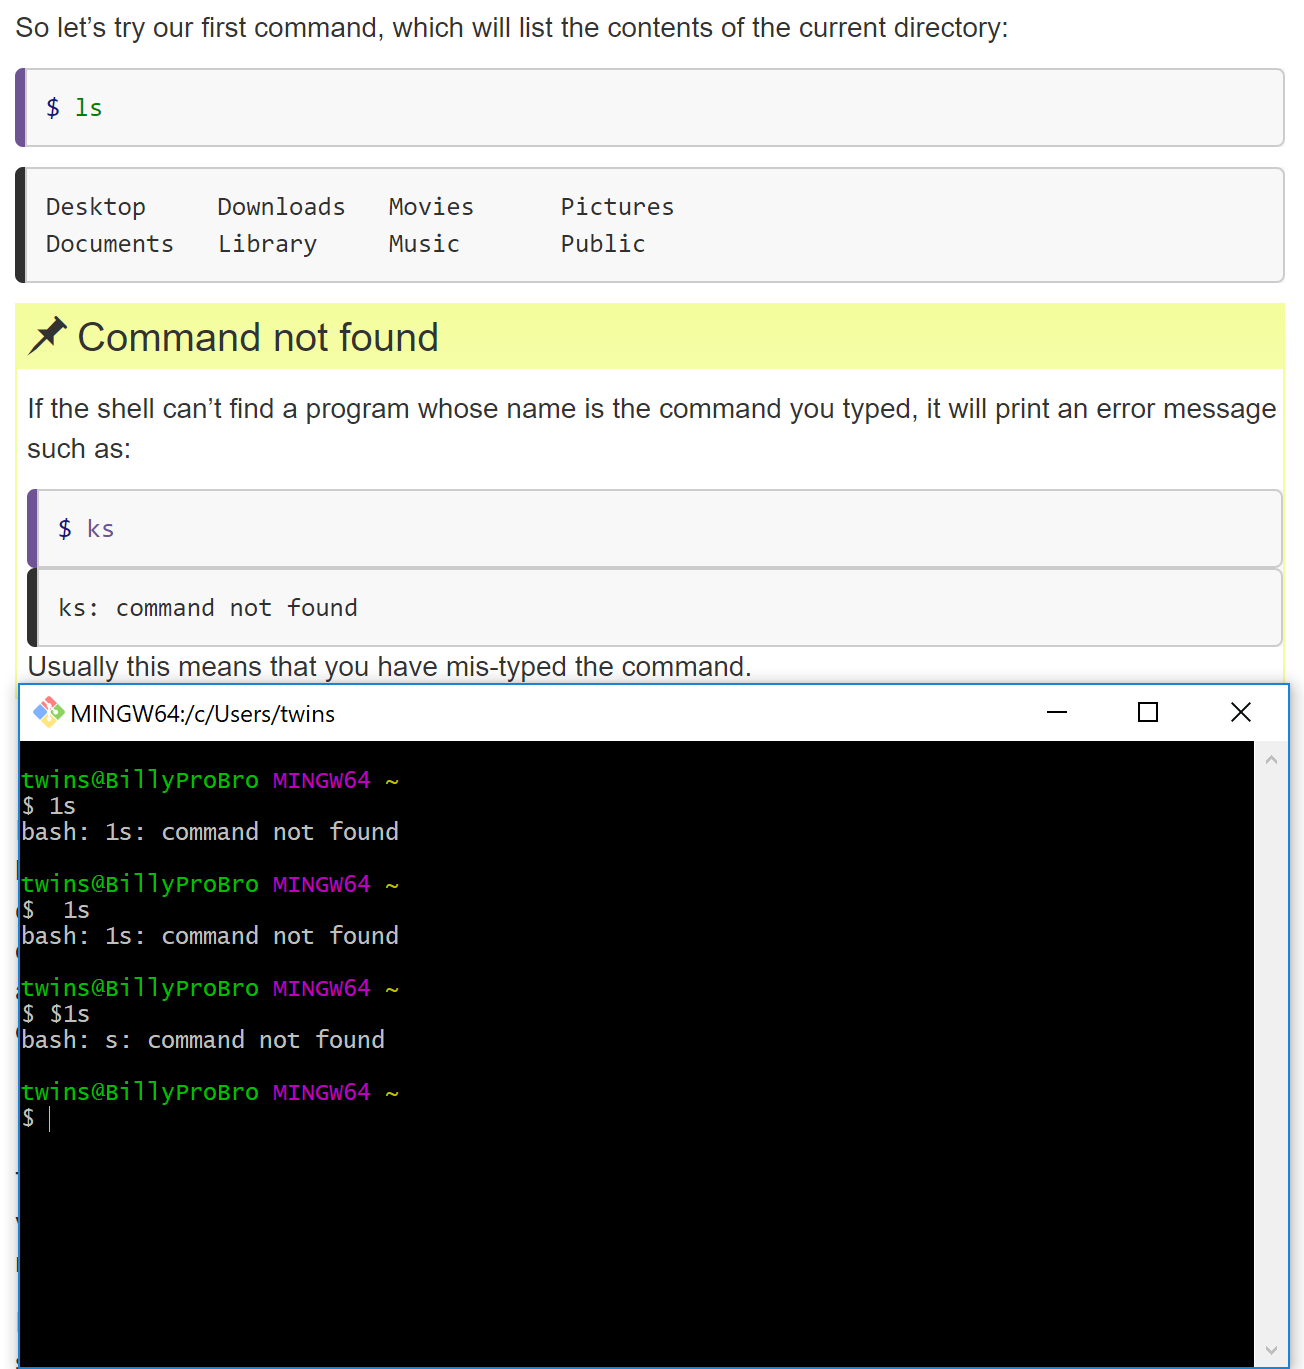
\includegraphics[scale=0.8]{imgcommandnotfound.PNG}
\end{itemize}
\begin{itemize}
\renewcommand{\labelitemi}{}
\item \underline{Solution:}
\renewcommand{\labelitemi}{$\bullet$}
    \item Copy-pasted it into a document to discover the character is not a one but a lower-case L.
    \item So the command is LS? Why?
    \item \href{https://en.wikipedia.org/wiki/Ls}{Wikipedia} says it's short for "list". Welp, they did warn us this wasn't intuitive.
\end{itemize}

\newpage
\textbf{Is it difficult?} - ... Yes.

\textbf{Flexibility and automation} - Using shell grammar, you can handle large volumes of data automatically. CLIs are also the easiest way to interact with remote machines, supercomputers, clusters and clouds.

\textbf{Nelle's Pipeline: A Typical Problem}

Nelle Nemo's done a 6 month survey sampling gelatinous marine life. She has 1520 samples and must:
\begin{enumerate}
    \item Run each sample through an assay machine that will measure the relative abundance of 300 different proteins. The machine’s output for a single sample is a file with one line for each protein.
    \item Calculate statistics for each of the proteins separately using a program her supervisor wrote called \texttt{goostats}.
    \item Write up results. Her supervisor would really like her to do this by the end of the month so that her paper can appear in an upcoming special issue of Aquatic Goo Letters.
\end{enumerate}

Clicking each file and running \texttt{goostats} one-by-one in the Gooey is going to take weeks of work and give Nemo RSI. Ironically, a CLI is going to be more efficient at handling her Gooey samples. :D

\subsection{\href{http://swcarpentry.github.io/shell-novice/02-filedir/index.html}{\textbf{Navigating Files and Directories}}}

\color{gray}
\underline{Questions}

How can I move around on my computer?

How can I see what files and directories I have?

How can I specify the location of a file or directory on my computer?

\vspace{1em}
\underline{Objectives}

Explain the similarities and differences between a file and a directory.

Translate an absolute path into a relative path and vice versa.

Construct absolute and relative paths that identify specific files and directories.

Demonstrate the use of tab completion, and explain its advantages.
\color{black}

\vspace{1em}
The "file system" is the file \& directory manager of the OS. Creating/inspecting/renaming/deleting files \& directories can be done with shell commands.

We can see where we are with the command \texttt{pwd} (Print Working Directory). Trying the command myself, and I'm at my home directory.

The root directory can be referred to with just "/". The following names are the directories in nesting order, separated by slashes.

Typing command \texttt{ls} prints the names of files and directories in the CWD (Current Working Directory), and \texttt{-F} (a Flag) can be added after a space to mark files:

/ = directory

@ = link

* = exe

\newpage
\textbf{General syntax of a shell command}

In the case of \texttt{\$ ls -F /}\begin{itemize}
    \item \texttt{\$} is the \textbf{prompt}. 
    \item \texttt{ls} is the \textbf{command}.
    \item \texttt{-F} is an \textbf{option} (a type of \textbf{parameter}).
    \item \texttt{/} is an \textbf{argument} (a type of \textbf{parameter}).
\end{itemize}

Commands can be called with multiple parameters, but parameters aren't required. Spaces are required to separate each part, and parts may be case-sensitive.

\vspace{1em}
\textbf{Getting help}

\texttt{\$ls --help} provides a help option for a cheat sheet of available options. (\texttt{man ls} does not work, but this is apparently fine as long as \texttt{--help} works.)

\vspace{1em}
\color{gray}\begin{addmargin}[1cm]{0cm}
\underline{Exercise:}

What does the command ls do when used with the -l option? What about if you use both the -l and the -h option?

\color{black}

As it says in \texttt{--help}, it makes longer numbers easier to read for humans.

\end{addmargin}

\vspace{1em}
\color{gray}\begin{addmargin}[1cm]{0cm}
\underline{Exercise:}

The command \texttt{\$ls -R} lists the contents of directories recursively, i.e., lists their sub-directories, sub-sub-directories, and so on at each level. The command \texttt{\$ls -t} lists things by time of last change, with most recently changed files or directories first. In what order does \texttt{\$ls -R -t} display things?

\color{black}
Okay so, first of all, do NOT try this on the home directory, this is taking forever. 

I'm going to just close the CLI and reopen it.

I can't seem to change my location yet, but when I can I'll perform this exercise on a smaller folder. \textcolor{teal}{\small{- 9:50am: The command lists all files in all directories, with files organised by timestamp within directories. This is easier to see if you add the option \texttt{-l} to make timestamps visible.}}
\end{addmargin}
\vspace{1em}
\color{black}
\texttt{\$ ls -F Desktop} lists the files in a different directory - this time, the Desktop.

\texttt{\$ ls -F Desktop/data-shell} lists the files in Desktop/data-shell.

\texttt{\$ cd Desktop} changes the cwd to Desktop.

\texttt{\$ cd ..} to return to parent directory.

\texttt{\$ ls -F -a} includes the \texttt{-a} option to show All files and directories in cwd (\texttt{./}) and parent (\texttt{../}) directories.

You can combine options by listing them after a single \texttt{-}. E.g. \texttt{\$ ls -F -a} is an identical command to \texttt{\$ ls -Fa}

\texttt{\$ cd} returns you to home directory.

Although the guide suggests \texttt{\$ cd /Users/nelle/Desktop/data-shell} should take us to the data-shell directory, I can see from using \texttt{pwd} that in my case \texttt{\$ cd /c/Users} is required.

\texttt{\textasciitilde} = home directory (\texttt{\textasciitilde/Desktop} is identical to \texttt{/c/Users/twins/Desktop})

\texttt{-} = previous directory I was in (So \texttt{\$ cd -} takes you back a directory. Very handy.)

\vspace{0.5em}
\begin{addmargin}[1cm]{0cm}
\textcolor{gray}{\underline{Exercise:}\vspace{0.5em}\\Starting from /Users/amanda/data, which of the following commands could Amanda use to navigate to her home directory, which is /Users/amanda?
\begin{enumerate}
    \item \texttt{\$ cd .}
    \item \texttt{\$ cd /}
    \item \texttt{\$ cd /home/amanda}
    \item \texttt{\$ cd ../..}
    \item \texttt{\$ cd \textasciitilde}
    \item \texttt{\$ cd home}
    \item \texttt{\$ cd \textasciitilde/data/..}
    \item \texttt{\$ cd}
    \item \texttt{\$ cd ..}
\end{enumerate}}

I would guess only 5 and 9 would work. 

Testing them out, I can see 8 also works, I forgot that shortcut always takes you back to home directory. 7 also works, but is redundant.

\vspace{0.5em}
\textcolor{gray}{\underline{Exercise:}}
\begin{center}
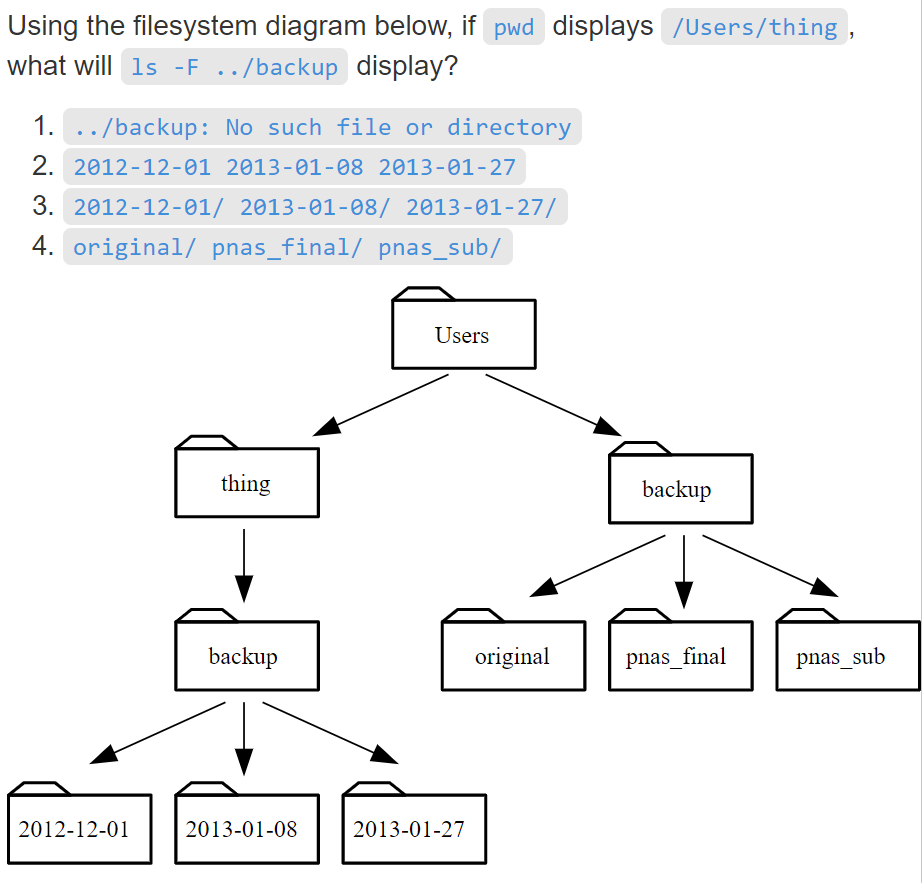
\includegraphics[scale=1]{imgrelativepathresolution.PNG}
\end{center}

Answer should be 4. Solution agrees.

\newpage
\textcolor{gray}{\underline{Exercise:}\vspace{0.5em}}
\begin{center}
\vspace{1em}
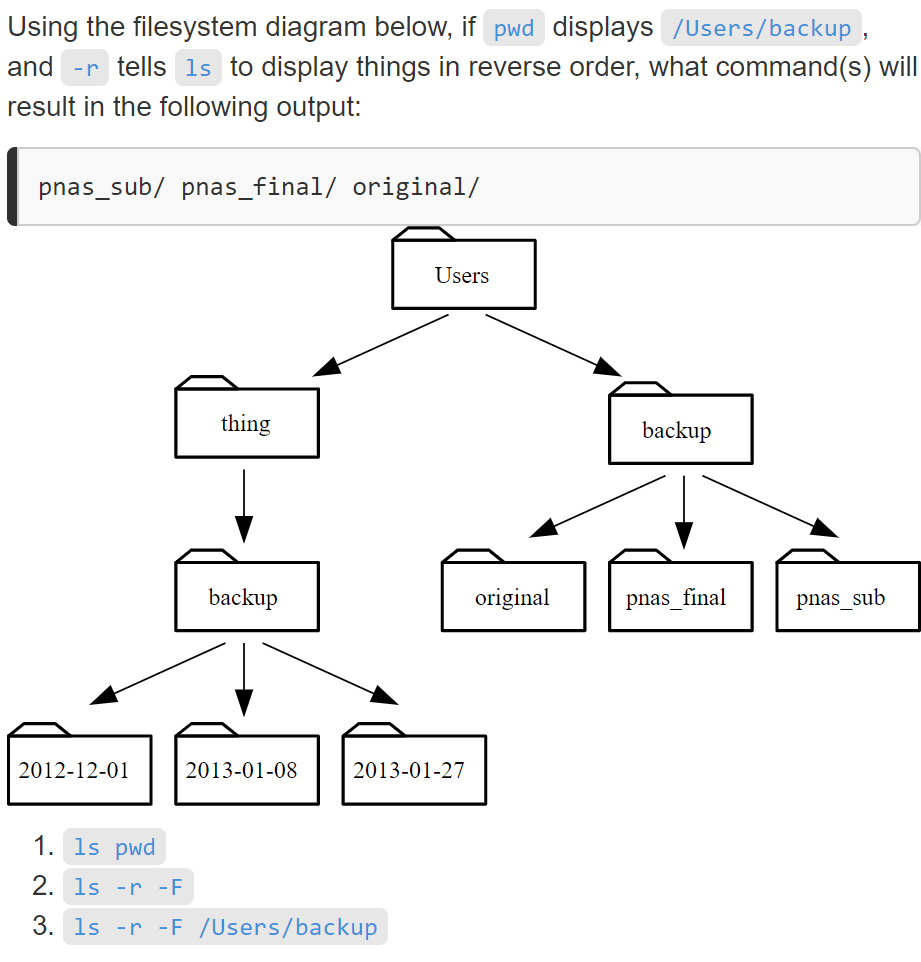
\includegraphics[scale=1]{imgreadingcomprehension.PNG}
\end{center}

I imagine 2 and 3 would work. 3 seems redundant.
\end{addmargin}

\newpage\section{29.08.19 - Proof of Concept: Elaboration I}

\subsection{Planning the Proof of Concept}

There are 3 semi-magic robots to choose from: a focus frame robot that keeps tabs on how much I'm writing in a digital workspace, a citation robot that manages citations for me, and a robot that lets me compare lyrics line-by-line easily. 

I am very attracted to making the first one because it's something I could reuse for every research project I do in future, and something that I suspect I could make within the semester, and something that I've never had a solution to before.

The citation robot would be great too but I'm seeing a lot of similar tools online, which would maybe make it easier for this semester as I could look to other codes for inspiration and edit changes. But if there are already solutions out there, it's not really that exciting to make another one.

The lyrics comparison robot is unique and could be useful for this specific project but would have really limited use in future. 
I'm going to go with the first robot, not only because of its value to me personally and reusability but also because I think in the time I have this semester I could easily extend or limit its required duties in order to increase or decrease the challenge.

For an elaboration on the PoC I just need to list the duties of the robot and work out how those duties would be possible.

Looking for technologies that could replicate some of these processes, I've found a short chapter on \href{https://en.wikibooks.org/wiki/LaTeX/Macros}{wikibooks} that discusses how to make macros and teach LaTeX "new tricks". It also says "LaTeX is a fairly high-level language compared to Plain TeX and thus is more limited." I'm not sure exactly what that means but it sounds like I might be making the robot out of "macro", either in LaTeX or TeX.

The more I look into macros the more it seems like everything I would do for this PoC would come down to creating, editing and extending this macro. 

Coming up with ways to "test" this process is arduous but a good exercise, because it's really made me think about how to chunk the problem and aim for the fastest way to fail possible. 

\newpage\section{30.08.19 - Data Carpentry: Unix Shell}
\subsection{\href{http://swcarpentry.github.io/shell-novice/03-create/index.html}{\textbf{Working With Files and Directories}}}

\color{gray}
\underline{Questions}

How can I create, copy, and delete files and directories?

How can I edit files?

\vspace{1em}
\underline{Objectives}

Create a directory hierarchy that matches a given diagram.

Create files in that hierarchy using an editor or by copying and renaming existing files.

Delete, copy and move specified files and/or directories.
\color{black}

\vspace{1em}
\textbf{Creating directories}

\texttt{\$ mkdir foldername} makes a folder called foldername in the cwd. - This is a good reason to not use spaces and special characters in file/directory names. If you're stuck with a name that does have a space, you have to surround it with quotes. E.g. \texttt{\$ cd "Billy's folder"}

\vspace{1em}
\textbf{Creating text files}

\texttt{\$ nano draft.txt} creates a text document in Nano, a basic text editor. There are other text editors like Vim or Notepad++, when you're ready to trade learning time for better utility.

Use the nano screen to write/edit the document, and use \textsuperscript{$\wedge$}O to "write out" (this means save, apparently). The shortcuts are at the bottom, and the carat \textsuperscript{$\wedge$} mark means Ctrl+. E.g. \textsuperscript{$\wedge$}X Exit means press Ctrl+X to exit.

\begin{addmargin}[1cm]{0cm}
\vspace{1em}
\color{gray}
\underline{Exercise:}

We have seen how to create text files using the nano editor. Now, try the following command: \texttt{\$ touch my\_file.txt}

\begin{enumerate}
    \item What did the touch command do? When you look at your current directory using the GUI file explorer, does the file show up?
    \item Use ls -l to inspect the files. How large is my\_file.txt?
    \item When might you want to create a file this way?
\end{enumerate}
\color{black}
\begin{enumerate}
    \item It seems to have made an empty file, it does show up on my Gooey.
    \item Looks like it's 0b
    \item Perhaps you need an empty file for another program to refer to, like how in spreadsheets you might need a zero in some cells rather than leaving the data empty? - Reading the solution, it seems that answer is more or less right. Some programs need the file to at least exist before they can populate it with information. 
\end{enumerate}
\end{addmargin}

\newpage\textbf{Moving files and directories}

\texttt{\$ mv draft.txt coffee.txt} uses move command to change the name of the file from "draft.txt" to "coffee.txt".

\texttt{\$ mv coffee.txt ..} would move the file to the cwd's parent directory.

Similarly, \texttt{\$ mv billys\_folder/coffee.txt .} would move coffee.txt from within billys\_folder to the cwd.

\begin{addmargin}[1cm]{0cm}
\vspace{1em}
\color{gray}
\underline{Exercise:}

After running the following commands, Jamie realizes that she put the files \texttt{sucrose.dat} and \texttt{maltose.dat} into the wrong folder:

\$ ls -F
 analyzed/ raw/

\$ ls -F analyzed
fructose.dat glucose.dat maltose.dat sucrose.dat

\$ cd raw/

Fill in the blanks to move these files to the current folder (i.e., the one she is currently in):

\$ mv \_\_\_/sucrose.dat  \_\_\_/maltose.dat \_\_\_

\vspace{1em}
\color{black}
After confirming on my own computer that you can move more than one file at once, the command should be: \texttt{\$ mv analyzed/sucrose.dat analyzed/maltose.dat .}, because "." represents the cwd.
\end{addmargin}

\vspace{1em}
\textbf{Copying files and directories}

\texttt{\$ cp billysfile.txt billysfilebackup.txt} copies the file rather than moves it. Naturally, you can determine the folder it copies to too, and copy entire directories to existing or new directories.

\textbf{Removing files and directories}

\texttt{\$ rm quotes.txt} to delete the file. Add option \texttt{-i} to use a prompt to check you're only deleting files you want to delete. Hardly useful for deleting one file but if you used \texttt{\$ rm -ri billysfolder} you would be prompted to agree to descend to billysfolder, then prompted for deleting each file within, one at a time, and then the folder itself.

\textbf{Wildcards}

\texttt{*} is a wildcard for zero or more characters.

\texttt{?} is a wildcard for a single character. 

\begin{addmargin}[1cm]{0cm}
\color{gray}
\vspace{1em}\underline{Exercise:}

When run in the molecules directory, which ls command(s) will produce 
\\\texttt{ethane.pdb methane.pdb}?
\\1. ls *t*ane.pdb
\\2. ls *t?ne.*
\\3. ls *t??ne.pdb
\\4. ls ethane.*
\color{black}

1 and 3. - Solution says not 1, because you would also catch octane.pdb and pentane.pdb. Fair point.

\color{gray}
\vspace{1em}\underline{Exercise:}

Sam has a directory containing calibration data, datasets, and descriptions of the datasets. Before heading off to another field trip, she wants to back up her data and send some datasets to her colleague Bob. Sam uses the following commands to get the job done.

Help Sam by filling in the blanks.
\begin{verbatim}
$ cp *dataset* backup/datasets
$ cp ____calibration____ backup/calibration
$ cp 2015-____-____ send_to_bob/all_november_files/
$ cp ____ send_to_bob/all_datasets_created_on_a_23rd/
\end{verbatim}

\color{black}
\begin{verbatim}
$ cp *dataset* backup/datasets
$ cp *calibration.txt backup/calibration
$ cp 2015-11-* send_to_bob/all_november_files/
$ cp *-23-dataset* send_to_bob/all_datasets_created_on_a_23rd/  
\end{verbatim}
\end{addmargin}

Solution agrees!

The other exercises were a bit too easy to be bothered journalling.

So far, although I can understand the purpose of using a CLI over the Gooey, it's hard to come up with any scenario where it could regularly be useful. Even copying/moving files can be done in a similar way in the Gooey by using the search function, selecting all of them, and copying/moving them where you wish.

\newpage\section{30.08.19 - LaTeX Error Clean Up}
\subsection{LaTeX}

Compiling this document returns 108 Errors, despite compiling and reading normally. I might be just good enough to fix a lot of these by now.

A lot of these errors are turning out to just be things like typing \# but forgetting to put a backslash behind it to escape the special character. Only 64 to go.

\subsubsection{\texorpdfstring{\underline{Error: Undefined Control Sequence}}{}}\label{error:er14}
\begin{itemize}
    \item\begin{verbatim}
<recently read> \nobullet
        
l.52\item\underline
        {Solution:}
            
The control sequence at the end of the top line of 
your error message was never \def'ed. If you have 
misspelled it, type `l' and the correct spelling. 
Otherwise just continue, and I'll forget whatever 
was undefined.
    \end{verbatim}
    \item So \$\textbackslash nobullet\$ is the problem? I think I might have just guessed to put that, since the normal type was \$\textbackslash bullet\$. 
\end{itemize}
\begin{itemize}
\renewcommand{\labelitemi}{}
    \item \underline{Solution:}
\end{itemize}
\renewcommand{\labelitemi}{$\bullet$}
\begin{itemize}
    \item Since the error message says it'll forget whatever was undefined, and \$\textbackslash nobullet\$ was undefined, so I figured leaving the curly brackets empty would be the same without the error.
    \item When that worked, I just replaced all instances of \{\$\textbackslash nobullet\$\} with \{\}. I was a bit worried about doing all of them at the same time like that so I copied the code into a new document before trying it. 
\end{itemize}

\subsubsection{\texorpdfstring{\underline{Error: Hyperref Token Not Allowed}}{}}\label{error:er15}
\begin{itemize}
    \item Even though the library of errors functions, it returns errors in coding the subsubsections they belong to. 
\end{itemize}
\begin{itemize}
\renewcommand{\labelitemi}{}
\item \underline{Solution:}
\renewcommand{\labelitemi}{$\bullet$}
    \item Apparently the issue is that the formatting of the subsubsection won't be convertible to PDF bookmarks, because they can't take formatting. So one solution would be to remove formatting from the subsubsection header.
    \item On the other hand, there is also the option to use \textbackslash texorpdfstring to separate headers for LaTeX and pdf bookmarks, that I found instructions for \href{https://tex.stackexchange.com/questions/53513/hyperref-token-not-allowed}{here}.
    \item Find \& Replace All can fix the entire document at once again.
\end{itemize}

\newpage\section{31.08.19 - Data Carpentry: Unix Shell}
\subsection{\href{http://swcarpentry.github.io/shell-novice/04-pipefilter/index.html}{\textbf{Pipes and Filters}}}

\color{gray}
\underline{Questions}

How can I combine existing commands to do new things?

\underline{Objectives}

Redirect a command’s output to a file.

Process a file instead of keyboard input using redirection.

Construct command pipelines with two or more stages.

Explain what usually happens if a program or pipeline isn’t given any input to process.

Explain Unix’s ‘small pieces, loosely joined’ philosophy.

\color{black}

\vspace{1em}
\textbf{Word Count}

\texttt{\$ wc *.pdb} lists number of lines, words, characters, in that order. \texttt{\$ wc -l *.pdb} does the same, to count lines only.


Intention: As there are only .pdb files in the folder, I attempted to do this without specifying *.pdb, to see if it would run on them all anyway

Action: \texttt{\$ wc -l}

Result: An alarming lack of result, no "loop" phase to return to the part where it awaits my next command.

\subsubsection{\texorpdfstring{\underline{Error: Shell: Does Not Print Or Loop}}{}}\label{error:er16}
\begin{itemize}
    \item After typing command \texttt{\$ wc -l}, REPL system does not Print or Loop. 
    \item This may be because \texttt{wc} is a command, \texttt{-l} is an option, but I haven't given any file to apply the command to.
\end{itemize}
\begin{itemize}
\renewcommand{\labelitemi}{}
\item \underline{Solution:}
\renewcommand{\labelitemi}{$\bullet$}
    \item Intention: I tried Ctrl+D to disconnect, and reopen GitBash.
    
    Action: \texttt{\textsuperscript{$\wedge$}D}
    
    Result: Actually it doesn't disconnect as usual, it Prints a numeral that counts the number of extra entries I've made since the error and Loops back for my next command.
    
    \item The next section of the lesson explains I can also use Ctrl+C to Cancel the command.
\end{itemize}

Intention: Following my original logic, if * is a wildcard then it should stand for .pdb as well as other letters in the file. 

Action: \texttt{\$ wc -l *}

Result: \texttt{*} works identically to \texttt{*.pdb}

\vspace{1em}
\textbf{Redirecting output to a file}

\texttt{>} Redirects output to a file instead of Print-ing it. 

\texttt{\$ wc -l *.pdb > lengths.txt}, for example, will print the line lengths to a new file called lengths.txt, or overwrite a file called lengths.txt if it already exists.

\newpage\textbf{Viewing contents of .txt file}

\texttt{\$ cat} is a command to concatenate and Print file contents.

Intention: It should work to concatenate and Print all these files by using *.

Action: \texttt{\$ cat *}

Result: Works.

Intention: The lesson suggests \texttt{\$ cat lengths.txt} but \texttt{*xt} should also work because it's the only .txt file.

Action: \texttt{\$ cat *xt}

Result: Also works. 

If there are many files, you can limit the contents to just one screenful with \texttt{\$ less lengths.txt}. Spacebar to go forward, \texttt{b} to go backward, \texttt{q} to quit.

\begin{addmargin}[1cm]{0cm}
\color{gray}
\vspace{1em}\underline{Exercise:}

If we run \texttt{sort} on a file the output is:
\begin{verbatim}
10
19
2
22
6
\end{verbatim}
If we run \texttt{sort -n} on the same input, we get this instead:
\begin{verbatim}
2
6
10
19
22
\end{verbatim}
Explain why \texttt{-n} has this effect.

\vspace{1em}
\color{black}
Presumably, \texttt{sort} arranges numbers lexicographically by default unless you add the option \texttt{-n} to request numeric arrangement.
\end{addmargin}

Intention: Sort lengths numerically and output to file called \texttt{sorted-lengths.txt}, retrieve first 3 lines to Print

Action: \texttt{\$ sort -n len* > sorted-lengths.txt}; \texttt{\$ head 3 sor*}

Result: \texttt{Cannot open '3' for reading: No such file or directory} It appears the shell has taken the 3 to be the file, and the 3 must be attached to the option of \texttt{-n}.

Intention: Attach 3 to \texttt{-n} option to retrieve first 3 lines to Print.

Action: \texttt{\$ head -n 3 sor*}

Result: Success.

\begin{addmargin}[1cm]{0cm}
\color{gray}
\underline{Exercise:}

Test the commands below to reveal the difference between the two operators:

\texttt{\$ echo hello > testfile01.txt} and \texttt{\$ echo hello >> testfile02.txt}

\color{black}
I can see from using \texttt{\$ cat tes*} that \texttt{>} overwrites the file while \texttt{>>} adds the echo to it.
\end{addmargin}

\newpage
\begin{addmargin}[1cm]{0cm}
\color{gray}
\vspace{1em}\underline{Exercise:}

We have already met the head command, which prints lines from the start of a file. tail is similar, but prints lines from the end of a file instead.

Consider the file data-shell/data/animals.txt. After these commands, select the answer that corresponds to the file animals-subset.txt:
\begin{verbatim}
$ head -n 3 animals.txt > animals-subset.txt
$ tail -n 2 animals.txt >> animals-subset.txt
\end{verbatim}
1. The first three lines of animals.txt
\\2. The last two lines of animals.txt
\\3. The first three lines and the last two lines of animals.txt
\\4. The second and third lines of animals.txt

\vspace{1em}
\color{black}

3. Solution agrees.
\end{addmargin}

\textbf{Pipes}

Vertical bar [\texttt{|}] is a pipe, it means the  output of the command left of the pipe is the input of the command to the right.

\begin{addmargin}[1cm]{0cm}
\color{gray}
\vspace{1em}\underline{Exercise:}

In our current directory, we want to find the 3 files which have the least number of lines. Which command listed below would work?

1. \texttt{\$ wc -l * > sort -n > head -n 3}
\\2. \texttt{\$ wc -l * | sort -n | head -n 1-3}
\\3. \texttt{\$ wc -l * | head -n 3 | sort -n}
\\4. \texttt{\$ wc -l * | sort -n | head -n 3}

\vspace{1em}
\color{black}

4. Solution agrees.
\end{addmargin}

\textbf{Filters}

Filters are programs like \texttt{wc} or \texttt{sort} that turn inputs to outputs.

\begin{addmargin}[1cm]{0cm}
\color{gray}
\vspace{1em}\underline{Exercise:}

A file called \texttt{animals.txt} contains the following data:

\begin{verbatim}
2012-11-05,deer
2012-11-05,rabbit
2012-11-05,raccoon
2012-11-06,rabbit
2012-11-06,deer
2012-11-06,fox
2012-11-07,rabbit
2012-11-07,bear
\end{verbatim}
What text passes through each of the pipes and the final redirect in the pipeline below?

\texttt{\$ cat animals.txt | head -n 5 | tail -n 3 | sort -r > final.txt}

\vspace{1em}
\color{black}

Print contents, then take the top five entries, and the bottom three entries (... so all of them then), sort in reverse order, and output the list in a file called \texttt{final.txt}. So it should create a document in the cwd with the same list backwards. Testing that out, that's not what happens! 
\end{addmargin}

{\subsubsection{\texorpdfstring{\underline{Error: Shell: Pipe Functionality}}{}}\label{error:er17}
\begin{itemize}
  \item Expected above exercise to result in reversed list of \texttt{animals.txt}, but returned \begin{verbatim}
    2012-11-06,rabbit
    2012-11-06,deer
    2012-11-05,raccoon
  \end{verbatim} 
\end{itemize}
\begin{itemize}
\renewcommand{\labelitemi}{}
\item \underline{Solution:}
\renewcommand{\labelitemi}{$\bullet$}
  \item `Print contents, then take the top five entries, \textit{and} the bottom three entries, sort in reverse order, and output to \texttt{final.txt}.' - `and' is where I went wrong. Pipe does `then', but never `and'.
  \item It should be: "Print contents, then take top five entries, THEN take bottom three entries of those five, then sort in reverse order, and output to \texttt{final.txt}.
  \item I was confused why rabbit and deer are in the same order as in the original file but now I'm seeing the original file was not in lexicographic order in the first place, it was sorted by date and unsorted past that. 
\end{itemize}}

\textbf{Displaying specific fields}

\texttt{cut} "cuts out" and isolates sections of each line. By default it expects fields to be separated by \texttt{tab}s but you can define a delimiter with \texttt{-d x}, where x is the character used as a delimiter.

\textbf{Displaying unique instances}

\texttt{uniq} command filters out adjacent identical lines in the file.

\begin{addmargin}[1cm]{0cm}
\color{gray}
\vspace{1em}\underline{Exercise:}

How could you extend this pipeline (using \texttt{uniq} and another command) to find out what animals the file contains (without any duplicates in their names)?

\texttt{\$ cut -d , -f 2 animals.txt}

\begin{verbatim}
2012-11-05,deer
2012-11-05,rabbit
2012-11-05,raccoon
2012-11-06,rabbit
2012-11-06,deer
2012-11-06,fox
2012-11-07,rabbit
2012-11-07,bear
\end{verbatim}

\color{black}

\texttt{\$ cut -d , -f 2 animals.txt | sort | uniq}

...? Success!

\end{addmargin}

\newpage
\textbf{Counting and displaying unique instances}

You can use the option \texttt{-c} with the command \texttt{uniq} to display a count of number of instances next to each unique item.

Intention: Display how many times each animal appears in \texttt{animals.txt}

Action: \texttt{\$ cut -d , -f 2 animals.txt | sort | uniq -c}

Result:\begin{verbatim}
    1 bear
    2 deer
    1 fox
    3 rabbit
    1 raccoon
\end{verbatim}


\begin{addmargin}[1cm]{0cm}
\color{gray}
\vspace{1em}\underline{Exercise:}

The wildcard expression \texttt{*[AB].txt} matches all files ending in \texttt{A.txt} or \texttt{B.txt}. Imagine you forgot about this.
\begin{enumerate}
    \item Can you match the same set of files with basic wildcard expressions that do not use the \texttt{[]} syntax? Hint: You may need more than one expression.
    \item The expression that you found and the expression from the lesson match the same set of files in this example. What is the small difference between the outputs?
    \item Under what circumstances would your new expression produce an error message where the original one would not?
\end{enumerate}

\color{black}
\begin{enumerate}
    \item You'd have to do \texttt{*A.txt} and \texttt{*B.txt} one after the other
    \item The outputs would be separate, so they wouldn't be in their order as a mixed list.
    \item ... I give up, I'm testing it out but I can't find any.
    
    Solution says "When there are no files ending in \texttt{A.txt}, or there are no files ending in \texttt{B.txt}." - I don't think that's true, it still works correctly if I type in \texttt{*[ABC].txt}. And \texttt{*[BC].txt} also works correctly, only returning the ones ending in B.txt. 
    - \textcolor{teal}{\small{4:02pm Apparently the `new' expression in question is the wildcard we've been using all week, and the `old' one is the one we've just learnt 
\begin{CJK}{UTF8}{}
\begin{Japanese}
\textbackslash\_(ツ)\_/
\end{Japanese}
\end{CJK}}}
\end{enumerate}
\end{addmargin}

\begin{addmargin}[1cm]{0cm}
\color{gray}
\underline{Exercise:}

Suppose you want to delete your processed data files, and only keep your raw files and processing script to save storage. The raw files end in .dat and the processed files end in .txt. Which of the following would remove all the processed data files, and only the processed data files?

1. rm ?.txt
\\2. rm *.txt
\\3. rm * .txt
\\4. rm *.*

\color{black}
2. Solution agrees.
\end{addmargin}

\newpage\section{02.09.19 - Data Carpentry: Unix Shell}
\subsection{\href{http://swcarpentry.github.io/shell-novice/05-loop/index.html}{\textbf{Loops}}}
\color{gray}
\underline{Questions}

How can I perform the same actions on many different files?

\vspace{1em}
\underline{Objectives}

Write a loop that applies one or more commands separately to each file in a set of files.

Trace the values taken on by a loop variable during execution of the loop.

Explain the difference between a variable’s name and its value.

Explain why spaces and some punctuation characters shouldn’t be used in file names.

Demonstrate how to see what commands have recently been executed.

Re-run recently executed commands without retyping them.

\color{black}
\vspace{1em}\textbf{Loops}

Loops repeat commands for each item in a list. They look like:

\texttt{\$ \textbf{for} thing \textbf{in} thinglist
\\\textbf{do}
\\    verbwith \$thing (pipes etc here)
\\\textbf{done}}

\textbf{Intention}: Try to get second line of each file

\textbf{Action}: \vspace{-1em}\begin{verbatim}
$ for filename in *
> do
> head -n 2 $filename | tail -n 1
> done
\end{verbatim}
\textbf{Result}: \vspace{-1em}\begin{verbatim}
CLASSIFICATION: basiliscus vulgaris
CLASSIFICATION: bos hominus
CLASSIFICATION: equus monoceros
\end{verbatim}

I had to do this twice because I tried to make an indentation in the loop with \texttt{tab} and the shell stopped functioning until I pressed \texttt{\textsuperscript{$\wedge$}C}.

It didn't need to be "filename", it could have been "x" or anything. Good news, you don't need to remember a bunch of types of thing, but keep yourself sane by making your labels intuitive.

\newpage\begin{addmargin}[1cm]{0cm}
\color{gray}
\vspace{1em}\underline{Exercise:}

What is the output of the following code?
\vspace{-1em}\begin{verbatim}
$ for datafile in *.pdb
> do
>    ls *.pdb
> done    
\end{verbatim}\vspace{-0.5em}
Now, what is the output of the following code?
\vspace{-1em}\begin{verbatim}
$ for datafile in *.pdb
> do
>	ls $datafile
> done
\end{verbatim}\vspace{-0.5em}
Why do these two loops give different outputs?

\color{black}
The first one says "for each file of .pdb, list all the .pdbs", so it prints all the .pdbs 6 times, once for each file.

The second code says "for each file of .pdb, list the file", so it prints the file for each file.
\end{addmargin}

\begin{addmargin}[1cm]{0cm}
\color{gray}
\vspace{1em}\underline{Exercise:}

What is the output of the following code?
\vspace{-1em}\begin{verbatim}
for alkanes in *.pdb
do
    echo $alkanes
    cat $alkanes > alkanes.pdb
done
\end{verbatim}\vspace{-0.5em}

\color{black}
"For each file of .pdb, print each file. For each file of .pdb, concatenate and print the text in a new file called alkanes.pdb". Because only one \textgreater  is used, the file is overwritten each time. 
\end{addmargin}

\begin{addmargin}[1cm]{0cm}
\color{gray}
\vspace{1em}\underline{Exercise:}

What is the output of the following code?
\vspace{-1em}\begin{verbatim}
for datafile in *.pdb
do
    cat $datafile >> all.pdb
done
\end{verbatim}\vspace{-0.5em}

\color{black}
"For each file of .pdb, concatenate and print the text additively in a new file called all.pdb". Because two \textgreater\textgreater are used, the file has text of each file. 
\end{addmargin}

\textbf{Using echo}

A lot of loops you use may do something you can't see the effect of quickly. You could just check every time you've done something that it's done what you expected, but if your brain can handle breaking a tiny bit further to put \texttt{echo} at the beginning, you can also see the program's report of what it's done. 

Below is a screenshot of me testing if my code
\vspace{-1em}\begin{verbatim}
$ for filename in *.dat
> do
>     cp $filename original-$filename
> done
\end{verbatim}\vspace{-1em}
worked, once the easy verbose way, and once the concise way.

\begin{center}
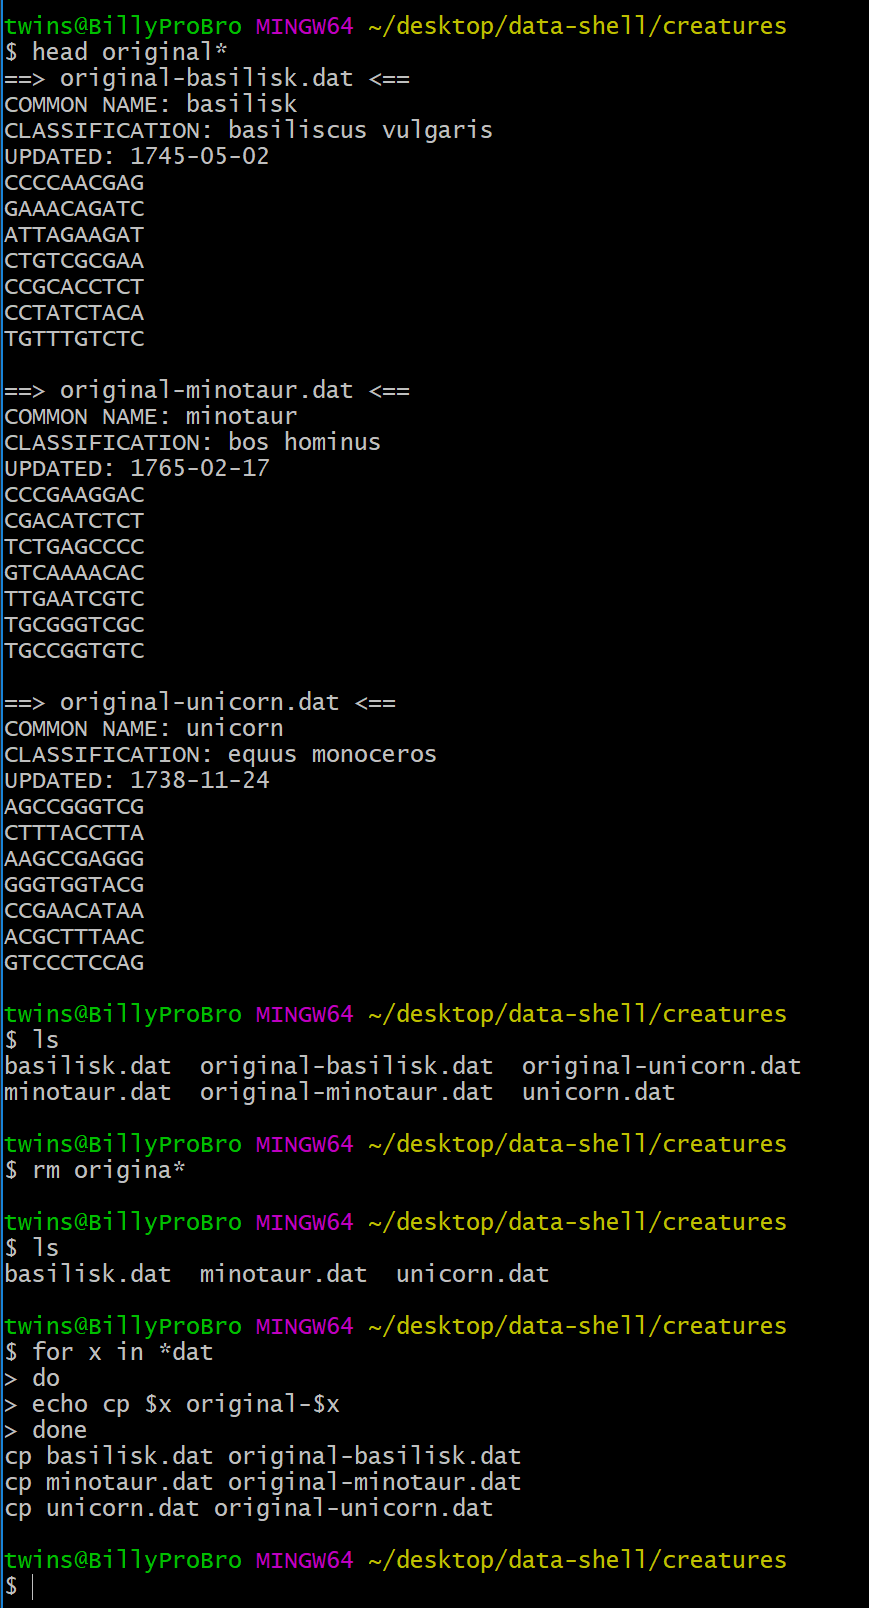
\includegraphics[scale=1]{imgusingecho.PNG}    
\end{center}

The best part is that if the program is taking ages to run you can see what it's up to and have an idea if you have time to make a coffee.

You can also use \texttt{echo} to get an idea of what the real command is going to do to what files.

\newpage\begin{addmargin}[1cm]{0cm}
\color{gray}
\vspace{1em}\underline{Exercise:}

What is the difference between the two loops below, and which one would we want to run to preview what will happen?
\vspace{-1em}\begin{verbatim}
$ for file in *.pdb
> do
>   echo analyze $file > analyzed-$file
> done

$ for file in *.pdb
> do
>   echo "analyze $file > analyzed-$file"
> done
\end{verbatim}\vspace{-0.5em}
\color{black}
I don't know. We haven't done quotation marks yet. I also don't know what the command "analyze" does yet, presumably that's a program. 

I guess in Version 1, it says "for every file of *pdb, print the fact that you're running the analyze program on each file and outputting the result in a file called "analyzed-[whatever the filename was]"".

Maybe Version 2 would just print what would happen without executing it, or perhaps it would literally print "analyze \$file $>$ analyzed-\$file"

Testing it on Nelle's NENE documents, I can see the quotes just show how the loop would apply to each file without executing it.
\end{addmargin}

\vspace{1em}
\textbf{History shortcuts}

Ctrl-R enters a history search mode “reverse-i-search” and finds the most recent command in your history that matches the text you enter next. Press Ctrl-R more times to search for earlier matches.

!! retrieves the immediately preceding command

!\$ retrieves the last word of the last command. That’s useful more often than you might expect: after bash goostats NENE01729B.txt stats-NENE01729B.txt, you can type \texttt{less !\$} to look at the file stats-NENE01729B.txt, which is quicker than doing up-arrow and editing the command-line.

\vspace{1em}
\textbf{Nested loops}

\begin{addmargin}[1cm]{0cm}
\color{gray}
\underline{Exercise:}

What would be the result of the following code:
\vspace{-1em}\begin{verbatim}
$ for species in cubane ethane methane
> do
>     for temperature in 25 30 37 40
>     do
>         mkdir $species-$temperature
>     done
> done
\end{verbatim}\vspace{-0.5em}
\color{black}
I really don't know, there aren't any files called 25 30 37 40. I don't know what those numbers could be. There are also no files called cubane ethane methane, I would have thought you needed .pdb. 

Testing it myself. I got those four numbered directories for each file. Okay... so the code said...

"for every file of cubane/ethane/methane, make a directory (called file-number) for every number of 25/30/37/40"

I guess I get that. I would never have guessed it without testing though.
\end{addmargin}

\newpage\section{03.09.19 - Data Carpentry: Unix Shell}
\subsection{\href{http://swcarpentry.github.io/shell-novice/06-script/index.html}{\textbf{Shell Scripts}}}
\color{gray}
\underline{Questions}

How can I save and re-use commands?

\underline{Objectives}

Write a shell script that runs a command or series of commands for a fixed set of files.

Run a shell script from the command line.

Write a shell script that operates on a set of files defined by the user on the command line.

Create pipelines that include shell scripts you, and others, have written.
\color{black}

\vspace{1em}
\textbf{Shell Scripts}

Shell scripts are a bunch of commands saved in a file to be re-run later when you type a single command word. 

\texttt{\$ nano newscript.sh} opens nano. Type in the script, then \texttt{\textsuperscript{$\wedge$}O} to save ("write out") to the folder to be run in, \texttt{\textsuperscript{$\wedge$}X} to exit, \texttt{\$ bash newscript.sh} to run.

\textbf{Argument Placeholders}

In the .sh script, you can use \texttt{"\$1"} and further numbers to indicate 1st/2nd/etc argument.

If you wanted to get the middle 50 lines from your 150-line data sheets: \texttt{head -n 100 "\$1" | tail -n 50} To run: \texttt{\$ bash newscript.sh desiredfile.txt} - the quotes around the \$1 is to get around the same issue as names with spaces.

To take this further and make it more customisable, the .sh script could be \texttt{head -n "\$2" "\$1" | tail -n "\$3"} To run: \texttt{\$ bash newscript.sh desiredfile.txt 100 50} or whatever numbers you'd like to run.

To keep yourself sane, add comments with \#; 
\\\texttt{\# For selecting lines from the middle of a document}
\\\texttt{\# Usage: \$ bash newscript.sh desiredfile.txt num\_oflastline num\_oflines}

If you need infinite arguments, you can use "\$@". Lesson example:
\vspace{-1em}\begin{verbatim}
    $ nano sorted.sh
    # Sort files by their length.
    # Usage: bash sorted.sh one_or_more_filenames wc -l "$@" | sort -n
    $ bash sorted.sh *.pdb ../creatures/*.dat
\end{verbatim}\vspace{-1em} This is a good example of when you might need multiple arguments because * would not be enough when they're in different locations.

\begin{addmargin}[1cm]{0cm}
\color{gray}
\vspace{1em}\underline{Exercise:}

Write a shell script called species.sh that takes any number of filenames as command-line arguments, and uses a variation of the above command to print a list of the unique species appearing in each of those files separately.
\color{black}

\vspace{-1em}\begin{verbatim}
# Outputs unique items in desired field of any csv files
# To use: $ bash species.sh commasep.file num_offield
cut -d , -f "$2" "$1" | sort | uniq
\end{verbatim}\vspace{-0.5em}
This works, but the solution has a different answer using "\$@", so re-reading the question I guess it means any number of filenames \textit{at once}. I'll try again. Does using "\$@" exclude me from using "\$1"? It must, right? Well the user is stuck with the second field then.
\vspace{-1em}\begin{verbatim}
# Outputs unique items in the second field of any number of csv files
# To use: $ bash species.sh commasep.file num_offield
cut -d , -f 2 "$@" | sort | uniq
\end{verbatim}\vspace{-1em}
Okay the solution is still different but just because they did something fancier:
\vspace{-1em}\color{gray}\begin{verbatim}
# Loop over all files
for file in $@
do
    echo "Unique species in $file:"
    # Extract species names
    cut -d , -f 2 $file | sort | uniq
done
\end{verbatim}\color{black}\vspace{-0.5em}
This is better just because when I run that, it'll be way more intuitive to understand what I'm reading. This is a good practice to get into, \texttt{echo}-ing what's about to happen in the code.
\end{addmargin}

\vspace{0.5em}\textbf{Recording the awesome thing you did to a script}

If you've done something correctly and want to make a script out of it to recreate it/recreate it for other files, you can do: \texttt{\$ history | tail -n 5 > scripttoupdatelog.sh} or however many lines to put your stuff in the script. Then you just need to edit out the line numbers and make the code fit your needs.

\begin{addmargin}[1cm]{0cm}
\color{gray}
\underline{Exercise:}

In the \texttt{molecules} directory, imagine you have a shell script called \texttt{script.sh} containing the following commands:

\vspace{-1em}\begin{verbatim}
head -n $2 $1
tail -n $3 $1
\end{verbatim}\vspace{-1em}
While you are in the \texttt{molecules} directory, you type the following command:
\vspace{-1em}\begin{verbatim}
bash script.sh '*.pdb' 1 1
\end{verbatim}\vspace{-1em}
Which of the following outputs would you expect to see?

\begin{enumerate}\vspace{-0.5em}
\item All of the lines between the first and the last lines of each file ending in .pdb in the molecules directory
\item The first and the last line of each file ending in .pdb in the molecules directory
\item The first and the last line of each file in the molecules directory
\item An error because of the quotes around *.pdb
\end{enumerate}

\color{black}\vspace{-0.5em}
The script says 
\\\texttt{head -n 1 '*.pdb'}
\\\texttt{tail -n 1 '*.pdb'}
\\So I guess it would be 2. I don't think the quotes are a problem, but it would have been easier to include the quotes in the script rather than the run command.
\end{addmargin}

\newpage\begin{addmargin}[1cm]{0cm}
\color{gray}
\underline{Exercise:}

Write a shell script called \texttt{longest.sh} that takes the name of a directory and a filename extension as its arguments, and prints out the name of the file with the most lines in that directory with that extension. For example:

\texttt{\$ bash longest.sh /tmp/data pdb} 

would print the name of the \texttt{.pdb} file in \texttt{/tmp/data} that has the most lines.

\vspace{1em}
\color{black}
Wow. Tough. 

\textbf{Intention:} First I want to know what file is the longest.

\textbf{Action:} \texttt{\$ wc -l * | sort}

\textbf{Result:} The full list of files with the longest at the bottom.

\vspace{1em}
\textbf{Intention:} Get that file

\textbf{Action:} \texttt{\$ wc -l * | sort | tail -n 1}

\textbf{Result:} \texttt{5118 total} 
- oh right. So it's the second-last line actually.

\textbf{Action:} \texttt{\$ wc -l * | sort | tail -n 2 | head -n 1}

\textbf{Result:} \texttt{300 NENE02043B.txt} 
Great!

\vspace{1em}
\textbf{Intention:} Getting there with a directory

\textbf{Action:} \texttt{\$ wc -l ~/desktop/data-shell* *.* | sort | tail -n 2 | head -n 1
}

\textbf{Result:} \texttt{wc: /c/Users/twins/desktop/data-shell: Is a directory
\\    300 NENE02043B.txt} - seems suspiciously functional. Fluke? 

\vspace{1em}
\textbf{Intention:} I'll test it on my own desktop.

\textbf{Action:} \texttt{\$ wc -l ~/desktop/* *.* | sort | tail -n 2 | head -n 1
}

\textbf{Result:}
\vspace{-1em}\begin{verbatim}
wc: /c/Users/twins/desktop/data-shell: Is a directory
wc: /c/Users/twins/desktop/emulators: Is a directory
wc: '/c/Users/twins/desktop/Learn French': Is a directory
wc: '/c/Users/twins/desktop/new 3ds crack': Is a directory
   6432200 /c/Users/twins/desktop/SL Training 2.zip
\end{verbatim}\vspace{-1em}
Hunh! I have a couple of other folders that didn't make the list, like 'SL Training 1.zip', I wonder why. But that is a very believable result, that training course is my weekend job and it takes a weekend to get through.

\textbf{Intention:} Write shell script.

\textbf{Action:} \texttt{\$ history | tail -n 2 > longest.sh}
\vspace{-1em}\begin{verbatim}
# Outputs line count and name of file with longest line count
# Usage: $ bash longest.sh directory ext
# e.g.   $ bash longest.sh desktop txt
wc -l "~/$1/" "*.$2" | sort | tail -n 2 | head -n 1
\end{verbatim}\vspace{-1em}

\textbf{Result:}
\vspace{-1em}\begin{verbatim}
$ bash longest.sh desktop/data-shell txt
wc: /c/Users/twins/desktop/data-shell/: Is a directory
    300 NENE02043B.txt
\end{verbatim}


AAAAYYYYY!
\end{addmargin}

\newpage

\begin{addmargin}[1cm]{0cm}
\color{gray}
\underline{Exercise:}

Explain what each of the following three scripts would do when run as \texttt{bash script1.sh *.pdb}, \texttt{bash script2.sh *.pdb}, and \texttt{bash script3.sh *.pdb} respectively.

\vspace{-1em}\begin{verbatim}
# Script 1
echo *.*

# Script 2
for filename in $1 $2 $3
do
    cat $filename
done

# Script 3
echo $@.pdb
\end{verbatim}

\color{black}\vspace{-0.5em}
Script 1: echo *.* *.pdb
\\This should print all files in the cwd of any extension, and all .pdb files.

Script 2: for x in *.pdb \$2 \$3; do cat \$x; done
\\This should print the contents of all .pdb files in the cwd, and perhaps return an error for \$2 and \$3.

Script 3: echo *.pdb.pdb
\\This should probably return an error, "file *.pdb.pdb not found" or something like that.

Solution says I'm wrong 3-for-3. So I'll just write the scripts and test them out.

\vspace{1em}
Script 1: echo *.*
\\*.pdb isn't registered at all because there's no \$1 in the shell script.
\\It prints all files in the cwd of any extension.

Script 2: for x in *.pdb *.pdb *.pdb; do cat \$x; done
\\Apparently the one argument just applies itself to all argument placeholders for some reason. Since everything else so far in the shell has never done anything without explicit and specific instruction, I really don't see why it would work this way.
\\It prints the contents of the first three files found to match *.pdb

Script 3: echo *.pdb.pdb
\\I forgot echo prints stuff even when it's not printing what you want.
\\It prints all the .pdb files, followed by .pdb.

Solution is now happy.
\end{addmargin}

\vspace{1em}
\textbf{Bash -x shellscript.sh}

When the script doesn't run as expected, you can add option -x to see each command as it's run, which will show you where the program is going wrong.



\newpage\section{05.10.19 - Data Carpentry: Unix Shell}
\subsection{\href{http://swcarpentry.github.io/shell-novice/07-find/index.html}{\textbf{Finding Things}}}
\color{gray}
\underline{Questions}

How can I find files?

How can I find things in files?

\underline{Objectives}

Use grep to select lines from text files that match simple patterns.

Use find to find files and directories whose names match simple patterns.

Use the output of one command as the command-line argument(s) to another command.

Explain what is meant by ‘text’ and ‘binary’ files, and why many common tools don’t handle the latter well.
\color{black}

\vspace{1em}\textbf{Grepping}

\textbf{GREP} = To do a \textbf{global} search for a \textbf{regular expression} and \textbf{print} it.

\texttt{\$ grep The example.txt}

Grepping "The" will return The, Thesis, Thesaurus etc. 

\texttt{\$ grep -w The example.txt}

Adding option \texttt{-w} limits matches by word boundaries, returning only The. For phrases with spaces, use quotation marks as always.

Adding option \texttt{-n} adds enumeration of what line the text appears.

Adding option \texttt{-i} makes search case-insensitive.

Adding option \texttt{-v} inverts search.

\begin{addmargin}[1cm]{0cm}
\color{gray}
\underline{Exercise:}

Which command would result in the following output: 

\texttt{and the presence of absence:}

1. \texttt{\$ grep "of" haiku.txt}
\\2. \texttt{\$ grep -E "of" haiku.txt}
\\3. \texttt{\$ grep -w "of" haiku.txt}
\\4. \texttt{\$ grep -i "of" haiku.txt}

\color{black}\vspace{0.5em}
1. Will return of and Software
\\2. I don't know what option \texttt{-E} does, it just says it does "PATTERN is an extended regular expression", whatever that means. Testing it out, it does still return both of and Software.
\\3. Correct answer
\\4. Search is case-insensitive, but that will still return Software.\end{addmargin}

Apparently adding option \texttt{-E} will prevent the shell from trying to interpret what's inside the quotes.

\texttt{\$ grep -E '\textsuperscript{$\wedge$}.o' haiku.txt} uses the \textsuperscript{$\wedge$} to anchor the match to the start of the line, the \texttt{.} to match a single character, and the \texttt{o} to match to an o.

\newpage \begin{addmargin}[1cm]{0cm}
\color{gray}
\underline{Exercise:}

The script should return one file called \texttt{species.txt} containing a list of dates and the number of that species seen on each date. For example using the data shown above, \texttt{rabbit.txt} would contain:

\vspace{-0.5em}\begin{verbatim}
2013-11-05,22
2013-11-06,19
\end{verbatim}\vspace{-0.5em}

\color{black}\vspace{-0.5em}
\begin{verbatim}
# Returns a file called examplespecies.txt containing a list of dates and the 
number of times that species was seen.
# Usage: $ bash species_datesseen.sh species directory 
# e.g.   $ bash species_datesseen.sh rabbit /animal-counts/
grep -w $1 -r $2 | cut -d : -f 2 | cut -d , -f 1,3 > $1.txt
\end{verbatim}
This script says to search the word "\$1" recursively in the "\$2" directory, get the second field (where fields are delimited by ":"), then get the first and third fields (where fields are delimited by ",") and print them to a text called "\$1.txt".
\end{addmargin}

\begin{addmargin}[1cm]{0cm}
\color{gray}
\underline{Exercise:}

You and your friend, having just finished reading \textit{Little Women} by Louisa May Alcott, are in an argument. Of the four sisters in the book, Jo, Meg, Beth, and Amy, your friend thinks that Jo was the most mentioned. You, however, are certain it was Amy. Luckily, you have a file \\\texttt{LittleWomen.txt} containing the full text of the novel \\(\texttt{data-shell/writing/data/LittleWomen.txt}). Using a for loop, how would you tabulate the number of times each of the four sisters is mentioned?

\color{black}\vspace{-0.5em}
\textbf{Intention:} First I need how many times Amy appears in the text

\textbf{Action:} \texttt{\$ grep -w Amy LittleWomen.txt}

\textbf{Result:} Every line in which she appears. But I only want every instance, without the rest of the line, so I can count the words in that.

{\subsubsection{\texorpdfstring{\underline{Error: Shell: Grepping Singular Words}}{}}\label{error:er18}
\begin{itemize}
  \item Expected above exercise to result in a list of found instances of searched word, but can only retrieve words in context of each line.
  \item \texttt{\$ grep wc -w Amy LittleWomen.txt} doesn't work; \texttt{\$ grep -w Amy LittleWomen.txt | wc -w} doesn't work; I've been trying for an hour and looking through my notes and I have no idea why the grep has to include the context or how to stop it.
  \item I'm cheating and looking at the solution.
\end{itemize}
\begin{itemize}
\renewcommand{\labelitemi}{}
\item \underline{Solution:}
\renewcommand{\labelitemi}{$\bullet$}
  \item Apparently, there's an option for -o that shows only the part of the line matching the grepped word. I have not been taught this option anywhere in the lesson so I will not assume I am supposed to be equipped to attempt exercises in future, and will check the solution if I don't immediately know the answer.
  \item Although this is unlikely to save me without specifically knowing where I'm going wrong, I could also use a command like \texttt{\$ grep --help} to look through ideas for options that might be helpful. For many commands, this --help is a list of possible options without actually telling you what they do, but it might help you guess.
\end{itemize}}



The solution was:
\vspace{-0.5em}\begin{verbatim}
for sis in Jo Meg Beth Amy
do
	echo $sis:
	grep -ow $sis LittleWomen.txt | wc -l
done
\end{verbatim}\end{addmargin}

\textbf{Finding}

\texttt{find} function is used to find files. \texttt{\$ find .} would find every single file and directory beginning with ".". Add \texttt{-type d} to find only directories, \texttt{-type f} to find only files, \texttt{-name '*.txt'} to find only files and directories containing .txt. (Note: '*.txt' is in quotes because asterisks are expanded before commands are run - without quotes you'll only get *.txts from the cwd.)

\texttt{\$ wc -l \$(find . -name '*.txt')} would first \texttt{find} all files in the cwd named *.txt, then wordcount the lines of those.

\begin{addmargin}[1cm]{0cm}
\color{gray}
\underline{Exercise:}

The -v option to grep inverts pattern matching, so that only lines which do not match the pattern are printed. Given that, which of the following commands will find all files in /data whose names end in s.txt (e.g., animals.txt or planets.txt), but do not contain the word net? Once you have thought about your answer, you can test the commands in the \texttt{data-shell} directory.

1. \texttt{find data -name '*s.txt' | grep -v net}
\\2. \texttt{find data -name *s.txt | grep -v net}
\\3. \texttt{grep -v "temp" \$(find data -name '*s.txt')}
\\4. None of the above.

\color{black}\vspace{0.5em}
I think the only one that would work from \texttt{/data-shell/} will be (1). (2) would find only cwd filenames ending in s.txt and I don't know what the plan was with (3).
\end{addmargin}

\begin{addmargin}[1cm]{0cm}
\color{gray}
\underline{Exercise:}

Write a short explanatory comment for the following shell script:

\texttt{wc -l \$(find . -name '*.dat') | sort -n}

\color{black}\vspace{0.5em}
This script finds all files in the cwd ending in .dat, sorts them lexicographically, and displays a line count of each file.
\end{addmargin}

\begin{addmargin}[1cm]{0cm}
\color{gray}
\underline{Exercise:}

The find command can be given several other criteria known as “tests” to locate files with specific attributes, such as creation time, size, permissions, or ownership. Use man find to explore these, and then write a single command to find all files in or below the current directory that are owned by the user ahmed and were modified in the last 24 hours.

\color{black}\vspace{0.5em}
\$ find . -type f -mtime -1 -user ahmed
\end{addmargin}

\newpage\section{08.11.19 - Data Carpentry: OpenRefine}
\subsection{\href{https://datacarpentry.org/openrefine-socialsci/02-working-with-openrefine/index.html}{\textbf{Working with OpenRefine}}}
\color{gray}
\underline{Questions}

How can we bring our data into OpenRefine?

How can we sort and summarize our data?

How can we find and correct errors in our raw data?

\underline{Objectives}

Create a new OpenRefine project from a CSV file.

Understand potential problems with file headers.

Use facets to summarize data from a column.

Use clustering to detect possible typing errors.

Understand that there are different clustering algorithms which might give different results.

Employ drop-downs to remove white spaces from cells.

Manipulate data using previous steps with undo/redo.

\color{black}

\vspace{2em}
\textbf{Facets}

A facet is essentially a filter with extra ability to display info on the data, clean and edit data and tags, sort information.

For instance, a text facet will count instances of each datum, a timeline facet will show a graph of the distribution of data over time, a numeric and scatterplot facets display graphs with drag and drop controls.

Custom facets are a range of different types of facets. For instance, you could see counts of items inside each datum by using \texttt{Custom text facet} and typing \texttt{value.split(";")}, assuming your values are separated by semicolons. 

Some of the default custom facets are:

\begin{itemize}
    \item Word facet - this breaks down text into words and counts the number of records each word appears in
    \item Duplicates facet - this results in a binary facet of ‘true’ or ‘false’. Rows appear in the ‘true’ facet if the value in the selected column is an exact match for a value in the same column in another row
    \item Text length facet - creates a numeric facet based on the length (number of characters) of the text in each row for the selected column. This can be useful for spotting incorrect or unusual data in a field where specific lengths are expected (e.g. if the values are expected to be years, any row with a text length more than 4 for that column is likely to be incorrect)
    \item Facet by blank - a binary facet of ‘true’ or ‘false’. Rows appear in the ‘true’ facet if they have no data present in that column. This is useful when looking for rows missing key data.
    

\end{itemize}

\newpage
\begin{addmargin}[1cm]{0cm}
\color{gray}
\underline{Exercise:}

1. Using faceting, find out how many different \texttt{interview\_date} values there are in the survey results.
\\2. Is the column formatted as Text or Date?
\\3. Use faceting to produce a timeline display for \texttt{interview\_date}. You will need to use Edit cells > Common transforms > To date to convert this column to dates.
\\4. During what period were most of the interviews collected?

\color{black}\vspace{1em}
1. 19 choices
\\2. As text
\\3. The timeline shows data collection was likely put on pause over the Christmas period.
\\4. Most of the interviews were collected in November.

\end{addmargin}

\vspace{1.5em}
\textbf{Clustering}

The cluster button merges data categories based on similar spelling, ngram appearance, or metaphony. It doesn't do it automatically so it's safe to check what will merge first.

\textbf{Transform}

\texttt{Edit Cells > Transform...} allows you to mass edit all data of the one category. For instance, if you type \texttt{value.replace("[","")}, it will replace all left square brackets in the values with nothing.

\vspace{1em}
\begin{addmargin}[1cm]{0cm}
\color{gray}
\underline{Exercise:}

1. Use this same strategy to remove the single quote marks ('), the right square brackets (]), and spaces from the \texttt{items\_owned} column.
\\2. Which two items are the most commonly owned? Which are the two least commonly owned?
\\3. Perform the same clean up steps and customized text faceting for the \texttt{months\_lack\_food} column. Which month(s) were farmers more likely to lack food?
\\4. Perform the same clean up steps for \texttt{months\_no\_water, liv\_owned, res\_change}, and the \texttt{no\_food\_mitigation} columns. Hint: To reuse a GREL command, click the History tab and then click Reuse next to the command you would like to apply to that column.

\color{black}\vspace{1em}
1. \texttt{value.replace("'", "")
\\value.replace("]", "")
\\value.replace(" ", "")}
\\2. Most commonly owned items were mobile phone and radio, least commonly owned were a computer or a car.
\\3. Sorting by count shows that farmers were most likely to lack food over November and surrounding months.
\\4. That was a lot of clicking. Hopefully there'll be a way to apply all those \texttt{value.replace}s at once.

\end{addmargin}

\vspace{1em}
\textbf{Trimming whitespace}

Trim spaces from the beginning and end of entries under common transforms.

\newpage
\subsection{\href{https://datacarpentry.org/openrefine-socialsci/03-filter-sort/index.html}{\textbf{Filtering and Sorting with OpenRefine}}}
\color{gray}
\underline{Questions}

How can we select only a subset of our data to work with?

How can we sort our data?

\underline{Objectives}

Filter to a subset of rows by text filter or include/exclude.

Sort table by a column.

Sort by multiple columns.

\color{black}

\vspace{1em}
\textbf{Filtering}

Clicking \texttt{Text filter} allows you to pick out the entries that contain text of your choosing

\begin{addmargin}[1cm]{0cm}
\color{gray}
\underline{Exercise:}

1. What roof types are selected by filtering \texttt{mabat}?
\\2. How would you restrict this to only one of the roof types?

\color{black}\vspace{0.5em}
1. Mabatisloping and mabatipitched
\\2. Use at least mabatip or mabatis. You can also click include on the entry you want

\color{gray}
\underline{Exercise:}

We discovered in an earlier lesson that the value for one of the village entries was given as 49. This is clearly wrong. By looking at the GPS coordinates for the entries of the other villages can we decide what village the data in that column was collected from?

\color{black}\vspace{0.5em}
Sorting by latitude and longitude can show that the village is amongst the other lats and longs for Chirodzo. If this was unclear (like it was between Chirodzo and another village), the interview date can be used to confirm if interviews were conducted in Chirodzo on that date.
\end{addmargin}

\newpage\section{12.11.19 - Data Carpentry: OpenRefine}\subsection{\href{https://datacarpentry.org/openrefine-socialsci/04-numbers/index.html}{\textbf{Examining Numbers in OpenRefine}}}
\color{gray}
\underline{Questions}

How can we convert a column from one data type to another?

How can we visualize relationships among columns?

\underline{Objectives}

Transform a text column into a number column.

Identify and modify non-numeric values in a column using facets.

\color{black}
\vspace{0.7em}
\textbf{Transforming to numbers}

Clicking \texttt{Edit cells > Common transforms… > To number} turns the cells in the column from lexicographic numeral data to numeric numeral data. This allows numeric manipulation and sorting.

\vspace{0.5em}
\begin{addmargin}[1cm]{0cm}
\color{gray}
\underline{Exercise:}

Transform three more columns, \texttt{no\_members, yrs\_liv}, and \texttt{buildings\_in\_compound}, from text to numbers. Can all columns be transformed to numbers? - Try it with \texttt{village} for example.

\color{black}\vspace{0.5em}
Transformation is allowed but there is no numeric data to transform. A notification observes that the change was applied (but to zero cells).

\color{gray}
\underline{Exercise:}

1. For a column you transformed to numbers, edit one or two cells, replacing the numbers with text (such as abc) or blank (no number or text).
\\2. Use the pulldown menu to apply a numeric facet to the column you edited. The facet will appear in the left panel.
\\3. Notice that there are several checkboxes in this facet: \texttt{Numeric, Non-numeric, Blank}, and \texttt{Error}. Below these are counts of the number of cells in each category. You should see checks for \texttt{Non-numeric} and \texttt{Blank} if you changed some values.
\\4. Experiment with checking or unchecking these boxes to select subsets of your data.

\color{black}\vspace{1em}
Selecting these subsets would be useful for data cleaning. Checking where fields have been left blank or have a non-numerical entry can avoid errors in maths like resulting averages.
\end{addmargin}

\vspace{-0.5em}\subsection{\href{https://datacarpentry.org/openrefine-socialsci/05-scripts/index.html}{\textbf{Using Scripts}}}
\color{gray}
\underline{Questions}

How can we document the data-cleaning steps we’ve applied to our data?

How can we apply these steps to additional data sets?

\underline{Objectives}

Describe how OpenRefine generates JSON code representing the work done in an analysis session.

Demonstrate ability to export this JSON code from OpenRefine.

Demonstrate ability to import a JSON code file to apply the analysis to another dataset.

\color{black}
\vspace{0.7em}
\textbf{JSON scripts}

While you clean and editing, OpenRefine is saving every change in a JavaScript Object Notation JSON script. If you have 20 files that need the same cleaning/fixing typos/changing blanks to zero/etc., the JSON script can be run on all of them.

In the \texttt{Undo / Redo} section, click \texttt{Extract...}, and select the steps that you want to apply to other datasets by clicking the check boxes. Save the code as a plain .txt file. Click \texttt{Apply...} to run it in another file.

\vspace{-0.5em}\subsection{\href{https://datacarpentry.org/openrefine-socialsci/06-saving/index.html}{\textbf{Exporting and Saving Data from OpenRefine}}}
\color{gray}
\underline{Questions}

How can we save and export our cleaned data from OpenRefine?

\underline{Objectives}

Save an OpenRefine project.

Export cleaned data from an OpenRefine project.

\color{black}
\vspace{0.7em}
\textbf{Saving and exporting}

OpenRefine saves continuously. To share data/cleaning steps to a collaborator or publisher, export the project. 

\vspace{0.5em}
\begin{addmargin}[1cm]{0cm}
\color{gray}
\underline{Exercise:}

1. Click the Export button in the top right and select Export project.
\\2. After you have expanded the file look at the files that appear in this folder. What files are here? What information do you think these files contain?.

\color{black}\vspace{0.5em}
A "history" folder which probably contains the log of changes made, and the data file. 

\end{addmargin}

\vspace{-0.5em}\subsection{\href{https://datacarpentry.org/openrefine-socialsci/05-scripts/index.html}{\textbf{Using Scripts}}}
\color{gray}
\underline{Questions}

How can we document the data-cleaning steps we’ve applied to our data?

How can we apply these steps to additional data sets?

\underline{Objectives}

Describe how OpenRefine generates JSON code representing the work done in an analysis session.

Demonstrate ability to export this JSON code from OpenRefine.

Demonstrate ability to import a JSON code file to apply the analysis to another dataset.

\color{black}
\vspace{0.7em}
\textbf{JSON scripts}

While you clean and editing, OpenRefine is saving every change in a JavaScript Object Notation JSON script. If you have 20 files that need the same cleaning/fixing typos/changing blanks to zero/etc., the JSON script can be run on all of them.

In the \texttt{Undo / Redo} section, click \texttt{Extract...}, and select the steps that you want to apply to other datasets by clicking the check boxes. Save the code as a plain .txt file. Click \texttt{Apply...} to run it in another file.

\textbf{Using online resources to get help with OpenRefine}

\href{https://github.com/OpenRefine/OpenRefine/wiki/Documentation-For-Users}{OpenRefine documentation Wiki site}

\newpage\section{12.11.19 - Data Carpentry: R for Social Scientists}

\subsection{\href{https://datacarpentry.org/r-socialsci/00-intro/index.html}{\textbf{Before we Start
}}}
\color{gray}
\underline{Questions}

How to find your way around RStudio?

How to interact with R?

How to manage your environment?

How to install packages?

\underline{Objectives}

Install latest version of R.

Install latest version of RStudio.

Navigate the RStudio GUI.

Install additional packages using the packages tab.

Install additional packages using R code.

\color{black}
\vspace{1em}

\textbf{What is R}

R is a programming language, but lots of people call IDEs (Integrated Development Environments) that are used to interact with the R software "R" too. It is open source and widely supported and troubleshot in the greater community.

R is designed for data analysis of spreadsheets, image analysis, time series, population genetics, a wide array of data types.

R finds results for your analysis based on your scripts rather than clicking, so you can be assured of a reproducible process if you add data to be analysed, and mistakes can be seen in code rather than guessed ad hoc. 

\textbf{What is RStudio}

RStudio is an IDE. Using an IDE we can write code, navigate the computer, inspect variables, generate plots, version control, develop packages, and more.

\vspace{0.5em}
\begin{addmargin}[1cm]{0cm}
\color{gray}
\underline{Exercise:}

1. Under the File menu, click \texttt{New project > New directory > New project}
\\2. Enter a name for this directory and choose a convenient location for it. This will be your working directory (e.g. \texttt{\textasciitilde/data-carpentry})
\\3. Click on \texttt{Create project}
\\4. Create a new file where we will type our scripts. Go to \texttt{File > New File > R script}. Click the save icon on your toolbar and save your script as "\texttt{script.R}”.

\color{black}\vspace{0.5em}

No errors.

\vspace{0.5em}
\color{gray}
\underline{Exercise:}

Use the install option from the packages tab to install the 'tidyverse' package.

\color{black}\vspace{0.5em}

No errors.
\end{addmargin}

\newpage\subsection{\href{https://datacarpentry.org/r-socialsci/01-intro-to-r/index.html}{Introduction to R}}

\color{gray}
\underline{Questions}

What data types are available in R?

What is an object?

How can values be initially assigned to variables of different data types?

What arithmetic and logical operators can be used?

How can subsets be extracted from vectors and data frames?

How does R treat missing values?

How can we deal with missing values in R?

\underline{Objectives}

Define the following terms as they relate to R: object, assign, call, function, arguments, options.

Assign values to objects in R.

Learn how to name objects.

Use comments to inform script.

Solve simple arithmetic operations in R.

Call functions and use arguments to change their default options.

Inspect the content of vectors and manipulate their content.

Subset and extract values from vectors.

Analyze vectors with missing data.

\color{black}
\vspace{1em}

\textbf{Creating objects}

Objects (or "variables" in other languages) are words that have values assigned to it with the assignment operator \texttt{<-} (alt+-).

\vspace{0.5em}
\begin{addmargin}[1cm]{0cm}
\color{gray}
\underline{Exercise:}

Objects can be used for arithmetic. Objects' values can be changed by assigning them new ones. This means that assigning a value to one object does not change the values of other objects.

1. Store the plot’s area in acres in a new object, \texttt{area\_acres}.
\\\texttt{area\_acres <- 2.47 * area\_hectares}
\\2. Then, change \texttt{area\_hectares} to 50.

What do you think is the current content of the object \texttt{area\_acres}? 123.5 or 6.175?

\color{black}\vspace{0.5em}

``Assigning a value to one object does not change the values of other objects." So it will still be 6.175. The \texttt{environment} pane also shows what values are currently assigned.

\end{addmargin}

\textbf{Comments}

Use \texttt{\#} to make comments. Use Ctrl+Shift+C to comment/uncomment entire selections at a time. 

\vspace{0.5em}
\begin{addmargin}[1cm]{0cm}
\color{gray}
\underline{Exercise:}

Create two variables \texttt{length} and \texttt{width} and assign them values. Create a third variable area and give it a value based on the current values of \texttt{length} and \texttt{width}. Show that changing the values of either \texttt{length} and \texttt{width} does not affect the value of area.

\color{black}\vspace{0.5em}

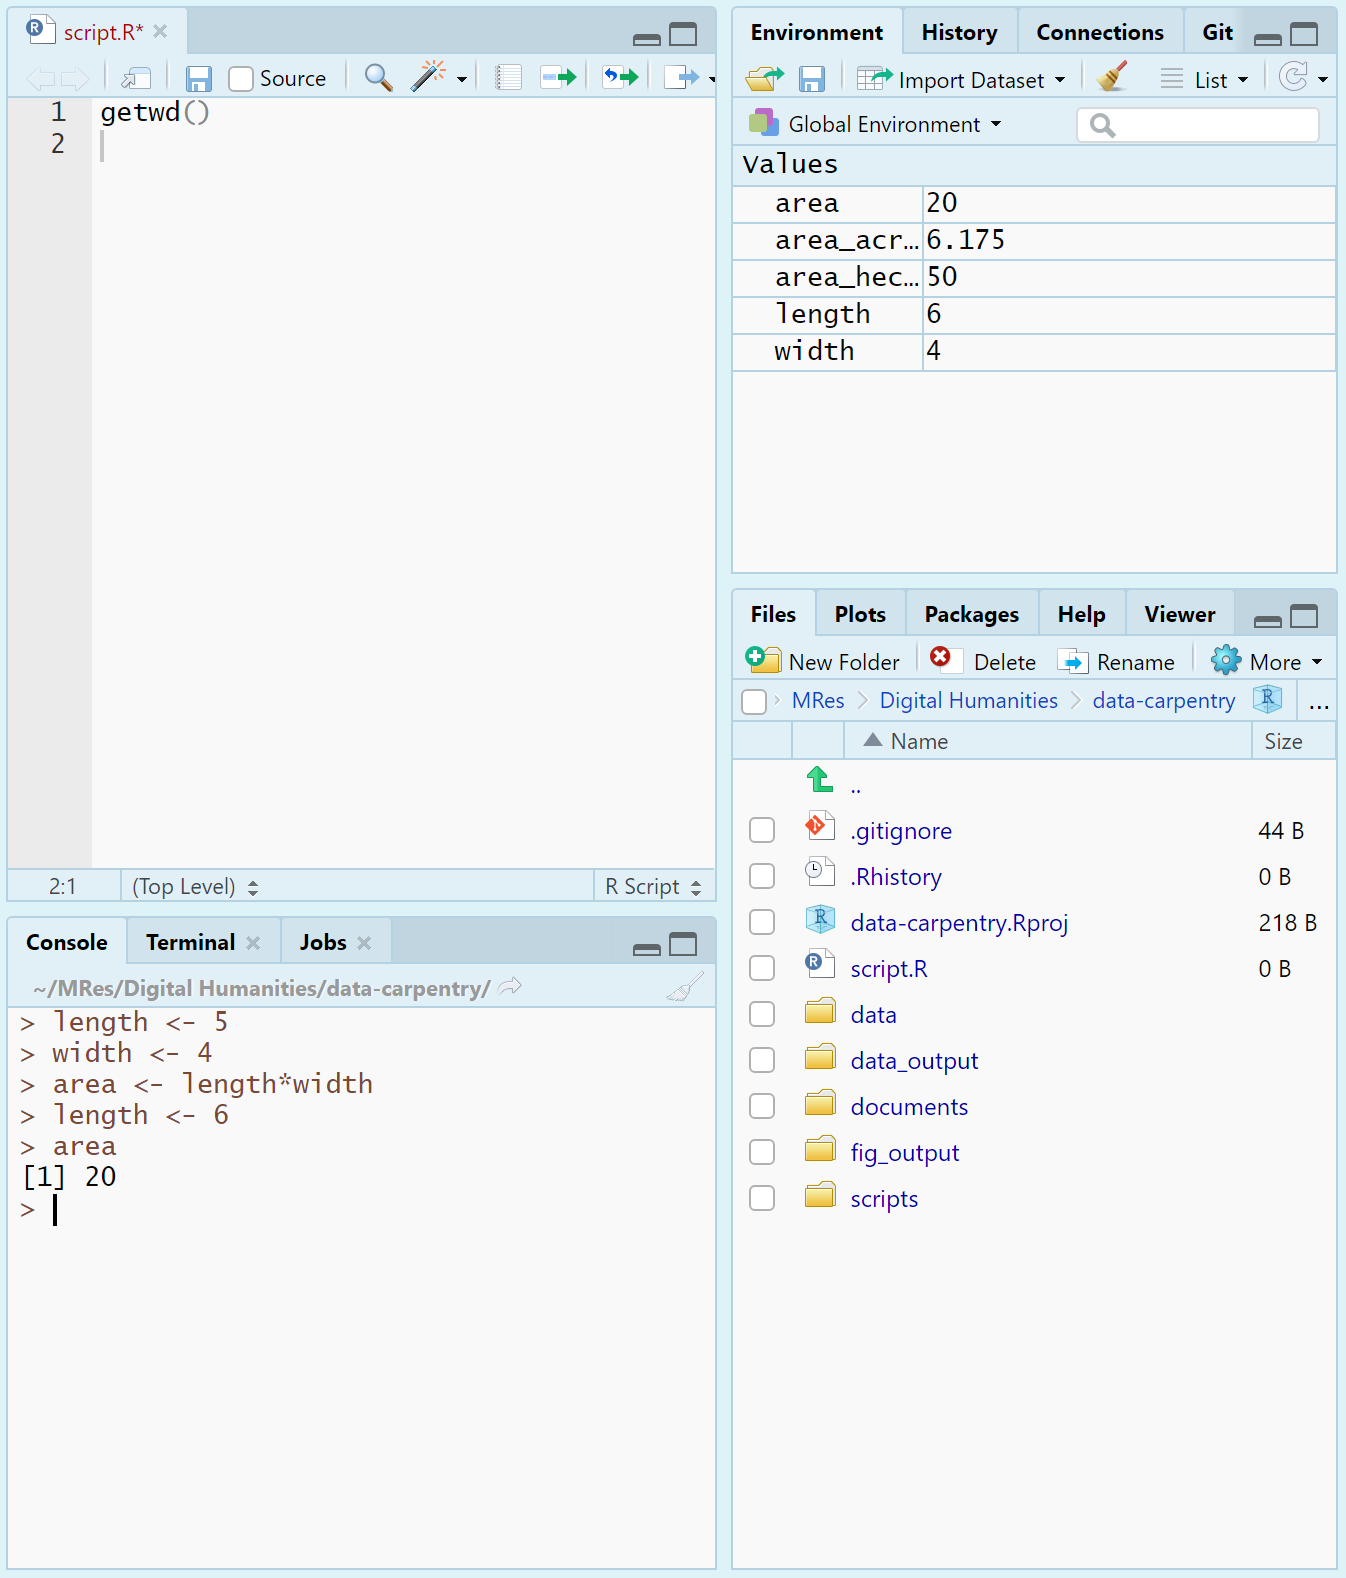
\includegraphics[scale=0.8]{imgrvariables.PNG}
\end{addmargin}

\textbf{Functions and their arguments}

Functions work roughly the same way they do in LaTeX, except using brackets after the function to assign arguments.

Use \texttt{args(nameoffunction)} to see what arguments the function can take. If you separate the values with commas RStudio will assume you meant arguments in the order they appear in, but you can specify arguments by name too. Use \texttt{?nameoffunction} for more detailed help.

\begin{verbatim}
    round(3.14159, 2)
    [1] 3.14

    round(digits = 2, x = 3.14159)
    [1] 3.14
\end{verbatim}

\textbf{Vectors}

A vector is a set of combined values set to an object with \texttt{c()}. The values can be numeric, character, integer, logical, complex, and raw. (Complex means 3 + 4i, for example, and raw is for a "bitstream" whatever that is) e.g. \texttt{hh\_members <- c(3, 7, 10, 6)} or \texttt{respondent\_wall\_type <- c("muddaub", "burntbricks", "sunbricks")}. The quotes are needed because otherwise R will think they're objects. This means you can use vectors as objects, too:
\begin{verbatim}
    possessions <- c("bicycle", "radio", "television")
    possessions <- c(possessions, "mobile_phone") # add to the end of the vector
    possessions <- c("car", possessions) # add to the beginning of the vector
\end{verbatim}

Use \texttt{length(vectorname)} to find out how many items are in the vector. Use \texttt{typeof(vectorname)} to find out what type it is. \texttt{str(vectorname)} to see the whole structure of the vector - also available in the Environment pane.

\vspace{0.5em}
\begin{addmargin}[1cm]{0cm}
\color{gray}
\underline{Exercise:}

We’ve seen that atomic vectors can be of type character, numeric (or double), integer, and logical. But what happens if we try to mix these types in a single vector? Why do you think that happens? 

\color{black}\vspace{0.5em}

Atomic vectors can only be one class. The different types take the common denominator as the type. TRUE/FALSE become 1 and 0 for numeric data, and numbers become a type of character. 

\end{addmargin}

\textbf{Subsetting vectors}

To extract values from a vector, type the indices you want in square brackets:

\vspace{-0.5em}\begin{verbatim}
    respondent_wall_type <- c("muddaub", "burntbricks", "sunbricks")
    respondent_wall_type[2]
        [1] "burntbricks"
    respondent_wall_type[c(3, 2)]
        [1] "sunbricks"   "burntbricks"
\end{verbatim}

\textbf{Conditional vectors}

You can also use logical vectors to extract values
\vspace{-0.5em}\begin{verbatim}
    hh_members <- c(3, 7, 10, 6)
    hh_members[c(TRUE, FALSE, TRUE, TRUE)]
        [1]  3 10  6
\end{verbatim}
\vspace{-0.5em}
You'd never want that though, it'd usually be the computer working out trues and falses for you. 
\vspace{-0.5em}\begin{verbatim}
    hh_members > 5 
        [1] FALSE  TRUE  TRUE  TRUE
    hh_members[hh_members > 5]
        [1]  7 10 6
\end{verbatim}
\vspace{-0.5em}
You can make multiple tests with \texttt{\&} (both conditions are true), or \texttt{|} (at least one condition is true). Use \texttt{\%in\%} to test if the string is found in the vector.
\vspace{-0.5em}\begin{verbatim}
    hh_members[hh_members < 3 | hh_members > 5]
        [1]  7 10  6
    hh_members[hh_members >= 7 & hh_members == 3]
        numeric(0)
    possessions <- c("car", "bicycle", "radio", "television", "mobile_phone")
    possessions[possessions == "car" | possessions == "bicycle"]
        [1] "car"     "bicycle"
    possessions %in% c("car", "bicycle", "motorcycle", "truck", "boat")
        [1]  TRUE  TRUE FALSE FALSE FALSE
    possessions[possessions %in% c("car", "bicycle", "motorcycle", "truck", "boat")]
        [1] "car"     "bicycle"
\end{verbatim}
\vspace{-0.5em}

\newpage \textbf{Missing data}

It's uncommon for programming languages to understand missing data, but R was designed for data analysis. Missing data is represented as \texttt{NA}, which will also be what displays if your function is being used on operations that include missing values. Add the argument \texttt{na.rm=TRUE} to calculate after removing missing values. Add \texttt{!is.na()} to isolate values other than NA. (\texttt{is.na()} would isolate NAs.)

\vspace{-0.5em}\begin{verbatim}
    rooms <- c(2, 1, 1, NA, 4)
    mean(rooms)
        [1] NA
    max(rooms)
        [1] NA
    mean(rooms, na.rm = TRUE)
        [1] 2
    max(rooms, na.rm = TRUE)
        [1] 4
    rooms[!is.na(rooms)]
        [1] 2 1 1 4
\end{verbatim}\vspace{-0.5em}

\vspace{0.5em}
\begin{addmargin}[1cm]{0cm}
\color{gray}
\underline{Exercise:}

1. Using this vector of rooms, create a new vector with the NAs removed.

\texttt{ rooms <- c(1, 2, 1, 1, NA, 3, 1, 3, 2, 1, 1, 8, 3, 1, NA, 1)}

2. Use the function median() to calculate the median of the rooms vector.

3. Use R to figure out how many households in the set use more than 2 rooms for sleeping.

\color{black}\vspace{0.5em}

{\subsubsection{\texorpdfstring{\underline{Error: R: Multiple Functions}}{}}\label{error:er19}
\begin{itemize}
  \vspace{-0.5em}\item \textbf{Intention:} To nest functions within a single command
  \vspace{-0.5em}\item \textbf{Action:} \texttt{rooms \%in\% [rooms >2]}
  \vspace{-0.5em}\item \textbf{Result:} \texttt{Error: unexpected '[' in "rooms \%in\% ["}
\end{itemize}
\begin{itemize}
\renewcommand{\labelitemi}{}
\item \underline{Solution:}
\renewcommand{\labelitemi}{$\bullet$}
  \item \textbf{Intention:} I need to create new objects with updated values in order to perform functions on them.
  \item \textbf{Action:} \vspace{-0.5em}\begin{verbatim}
      > rooms[!is.na(rooms)]
            [1] 1 2 1 1 3 1 3 2 1 1 8 3 1 1
        > roomswona <- rooms[!is.na(rooms)]
        > median(roomswona)
            [1] 1
        > roomswona[roomswona>2]
            [1] 3 3 8 3
        length(roomswona[roomswona>2])
            [1] 4
  \end{verbatim}
  \item \textbf{Result:} By assigning objects to each step of the process, I can perform functions on updated lists. And it's probably better not to tamper with your original list anyway - you may need it in its original form later.
\end{itemize}}

\end{addmargin}

\newpage\section{06.01.20 - Data Carpentry: R for Social Scientists}

\subsection{\href{https://datacarpentry.org/r-socialsci/02-starting-with-data/index.html}{\textbf{Starting with Data}}}
\color{gray}
\underline{Questions}

What is a data.frame?

How can I read a complete csv file into R?

How can I get basic summary information about my dataset?

How can I change the way R treats strings in my dataset?

Why would I want strings to be treated differently?

How are dates represented in R and how can I change the format?

\underline{Objectives}

Describe what a data frame is.

Load external data from a .csv file into a data frame.

Summarize the contents of a data frame.

Describe the difference between a factor and a string.

Convert between strings and factors.

Reorder and rename factors.

Change how character strings are handled in a data frame.

Examine and change date formats.
\color{black}
\vspace{1em}

\textbf{Loading the data in R}

Use \texttt{read\_csv()} to read a csv file, change the signal for na (or \texttt{read\_csv2} if delimiters are semicolons) and put it in a variable to use it.

E.g. \texttt{interviews <- read\_csv("data/SAFI\_clean.csv", na = "NULL")}

\textbf{Data Frames}

A data frame is a table where the columns are vectors (so single type of data e.g. character, logical, numeric) of equal length. Usually the frame is created by importing a spreadsheet with \texttt{read\_csv()} or \texttt{read\_table()}.

\textbf{Tibbles}

A tibble is a modern reimagining of the data frame, keeping what time has proven to be effective and throwing out what isn't. Tibbles are data frames that are lazy and surly; they do less (don't change variable names or types, don't do partial matching) and complain more (like when a variable doesn't exist), forcing you to confront problems ASAP to leave you with cleaner, more expressive code. When data is read with \texttt{read\_csv()}, it's stored in an object of class \texttt{tbl\_df}, \texttt{tbl}, and \texttt{data.frame}.

\vspace{0.5em}
\begin{addmargin}[1cm]{0cm}
\color{gray}
\underline{Exercise:}

1. Create a data frame (\texttt{interviews\_100}) containing only the data in row 100 of the interviews dataset.

2. Notice how \texttt{nrow()} gave you the number of rows in a data frame?

\begin{itemize}
    \item Use that number to pull out just that last row in the data frame.
    \item Compare that with what you see as the last row using \texttt{tail()} to make sure it’s meeting expectations.
    \item Pull out that last row using \texttt{nrow()} instead of the row number.
    \item Create a new data frame (\texttt{interviews\_last}) from that last row.
\end{itemize}

3. Use \texttt{nrow()} to extract the row that is in the middle of the data frame. Store the content of this row in an object named \texttt{interviews\_middle}.

Combine \texttt{nrow()} with the \texttt{\-} notation above to reproduce the behavior of \texttt{head(interviews)}, keeping just the first through 6th rows of the interviews dataset.
\end{addmargin}

\color{black}\vspace{0.5em}

\centering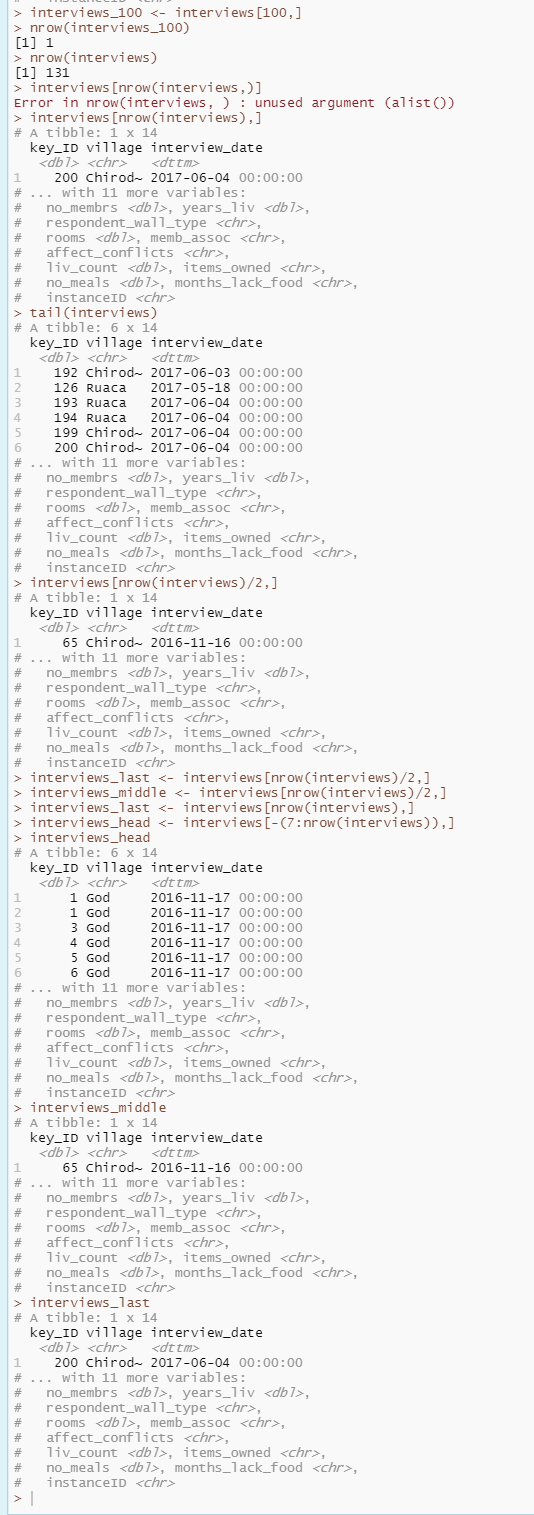
\includegraphics[scale=1]{imgdcrtibbles.PNG}

\flushleft\textbf{Factors}

A factor is a special data class for categorical data. Although they look like character vectors, they are treated as integer vectors. Factors can only contain pre-defined values known as "levels" which are always sorted alphabetically.

\texttt{levels(variable)} to see what levels, and \texttt{nlevels(variable)} to see number of levels.

The levels are given an integer based on alphabetical order, allowing categories to have an integer representation (useful for graphs etc), but are also self-descriptive.

You can manually change the levels, if it would make more sense. E.g. 

\texttt{respondentenglishcapacity <- factor(respondentenglishcapacity, levels = c("poor", "conversational", "fluent"))} 

This would make levels 1, 2, and 3 in that order instead of conversational - fluent - poor.

To rename a whole integer at once, encode the level of the factor. E.g. 

\texttt{levels(respondentenglishcapacity)[1] <- "developing"} 

This will change "poor" to "developing".

\vspace{1em}
\textbf{Converting factors to vectors}

To convert a factor to a character vector, use \texttt{as.character(respondentenglishcapacity)}

\texttt{as.numeric()} will just return the index values of the factor, leaving you with a list of 3 2 3 3 1 1 2 etc.

To convert to a numeric vector, \texttt{as.numeric(levels(yearcreated))[yearcreated]} is the recommended way to have a vector that looks like 1999, 1945, 2017, 2001 etc. 

The reason that works is that R gets the factor levels with \texttt{levels(yearcreated)}, convert the levels to their numeric index with \texttt{as.numeric()}, and then access the values using the underlying integer contained in \texttt{yearcreated} in square brackets.

\vspace{1em}\textbf{Plotting factors}

Use \texttt{plot()} to see the number of observations represented by each factor level. This will skip over NAs - rename NAs with \texttt{ispregnant[is.na(ispregant)] <- "Unknown"} if you want to include that information in your plot.


\vspace{0.5em}
\begin{addmargin}[1cm]{0cm}
\color{gray}
\underline{Exercise:}

1. Rename the levels of the factor to have the first letter in uppercase: “No”,”Undetermined”, and “Yes”.

2. Now that we have renamed the factor level to “Undetermined”, can you recreate the barplot such that “Undetermined” is last (after “Yes”)?

\color{black}\vspace{0.5em}
{\subsubsection{\texorpdfstring{\underline{Error: R: Renaming and Reordering Factors}}{}}\label{error:er20}
\begin{itemize}
    \item \textbf{Intention:} To rename and reorder "no", "undetermined", and "yes" to "No", "Yes", and "Undetermined" for a sensible graph.
    \item \textbf{Action:} \vspace{-1em}\begin{verbatim} 
> plot(memb_assoc)
> memb_assoc <- factor(memb_assoc, levels= c("No", "Yes", "Undetermined"))
> plot(memb_assoc)
    \end{verbatim}
    \item \textbf{Result:} The plot shows 0 responses for No, Yes, and Undetermined. I can see by calling \texttt{memb\_assoc} that every observation is now NA.
\end{itemize}
\begin{itemize}
\renewcommand{\labelitemi}{}
\item \underline{Solution:}
\renewcommand{\labelitemi}{$\bullet$}
      \item \textbf{Intention:} I need to restore the information to \texttt{memb\_assoc}, then change missing data to "undetermined" again, and rename the different levels.
    \item \textbf{Action:} \vspace{-1em}\begin{verbatim}
> memb_assoc <- interviews$memb_assoc
> memb_assoc[is.na(memb_assoc)] <- "undetermined"
> memb_assoc <- as.factor(memb_assoc)
> memb_assoc[1]
      \end{verbatim}\vspace{-2em}
      \item \textbf{Result:} \vspace{-1em}\begin{verbatim}
[1] undetermined
Levels: no undetermined yes
      \end{verbatim}\vspace{-2em} I realise that pulling [1] from the factor is actually giving me the first result, not the label of the first level. I need to rename the first level, not the results.
      \item \textbf{Action:} \vspace{-1em}\begin{verbatim}
> levels(memb_assoc)[1]
[1] "no"
> levels(memb_assoc)[1] <- "No"
> levels(memb_assoc)[2] <- "Yes"
> levels(memb_assoc)[3] <- "Undetermined"
> plot(memb_assoc)
      \end{verbatim}\vspace{-2em}
    \item \textbf{Result:} This is also wrong, I've accidentally renamed the missing data as "Yes" and the yeses as "Undetermined". I'm worried if I rename the missing data "Undetermined" then the factor may remove the the unused level, so I will rename it something different and rename the yeses correctly before fixing it. Then I can reorder the levels.
      \item \textbf{Action:} \vspace{-1em}\begin{verbatim}
> levels(memb_assoc)[2] <- "Undeterminedd"
> levels(memb_assoc)[3] <- "Yes"
> levels(memb_assoc)[2] <- "Undetermined"
> plot(memb_assoc)
> memb_assoc <- factor(memb_assoc, levels= c("No","Yes","Undetermined"))
> plot(memb_assoc)
      \end{verbatim}\vspace{-2em}
      \item\textbf{Result:} The graph displays correctly. 
\end{itemize}}      
\end{addmargin}
\centering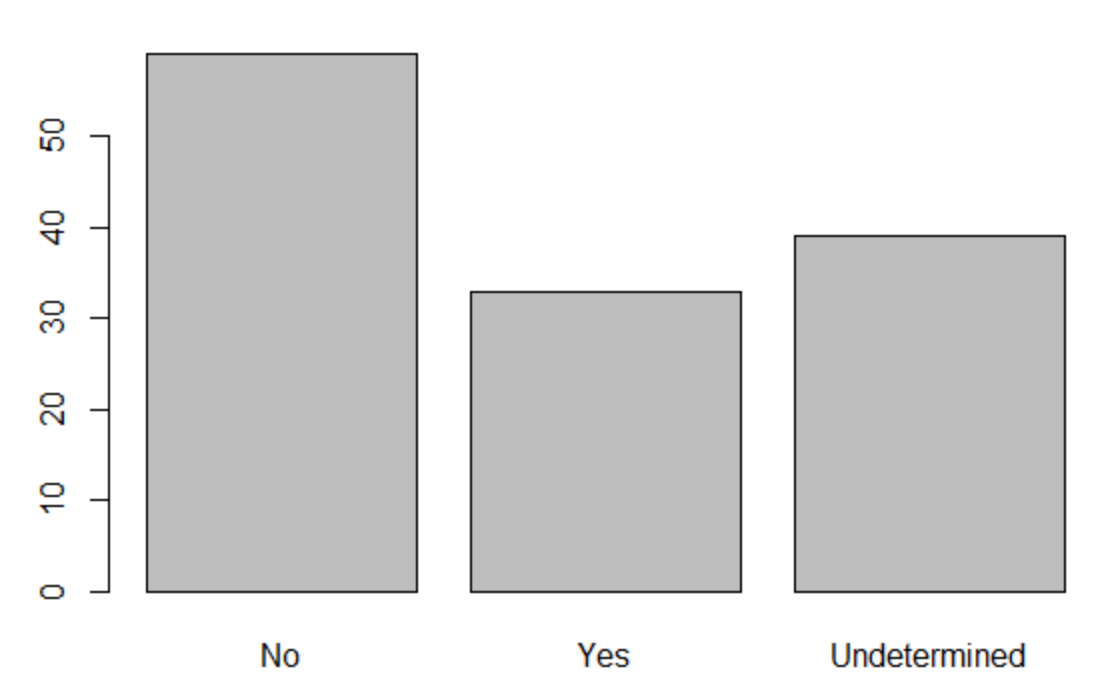
\includegraphics[scale=0.8]{imgdcrplot.PNG}

\newpage\flushleft\section{10.01.20 - Data Carpentry: R for Social Scientists}
\subsection{\href{https://datacarpentry.org/r-socialsci/03-dplyr-tidyr/index.html}{\textbf{Introducing dplyr and tidyr}}}
\color{gray}
\underline{Questions}

How can I select specific rows and/or columns from a data frame?

How can I combine multiple commands into a single command?

How can create new columns or remove existing columns from a data frame?

How can I reformat a dataframe to meet my needs?

\underline{Objectives}

Describe the purpose of an R package and the dplyr and tidyr packages.

Select certain columns in a data frame with the dplyr function \texttt{select}.

Select certain rows in a data frame according to filtering conditions with the dplyr function \texttt{filter}.

Link the output of one dplyr function to the input of another function with the ‘pipe’ operator \%\textgreater\%.

Add new columns to a data frame that are functions of existing columns with \texttt{mutate}.

Use the split-apply-combine concept for data analysis.

Use \texttt{summarize}, \texttt{group\_by}, and \texttt{count} to split a data frame into groups of observations, apply a summary statistics for each group, and then combine the results.

Describe the concept of a wide and a long table format and for which purpose those formats are useful.

Describe what key-value pairs are.

Reshape a data frame from long to wide format and back with the \texttt{spread} and \texttt{gather} commands from the tidyr package.

Export a data frame to a csv file.

\color{black}
\vspace{1em}

\textbf{Data Manipulation using \texttt{dplyr} and \texttt{tidyr}}

\texttt{dplyr} and \texttt{tidyr} are R packages written in C++ to manipulate data to different formats

\texttt{select()} selects columns of a data frame. First argument is the data frame, next arguments are which columns to keep

\texttt{filter()} chooses rows based on specific criteria. First argument is the data frame, next arguments are the responses to keep (e.g. village == "God")

Pipes take the object on the left and pass it as the first argument to the function on its right. \texttt{Ctrl+Shift+M} makes a pipe \texttt{\%\textgreater\%}


\vspace{0.5em}
\begin{addmargin}[1cm]{0cm}
\color{gray}
\underline{Exercise:}

Using pipes, subset the \texttt{interviews} data to include interviews where respondents were members of an irrigation association (\texttt{memb\_assoc}) and retain only the columns \texttt{affect\_conflicts}, \texttt{liv\_count}, and \texttt{no\_meals}.

\color{black}\vspace{0.5em}

\begin{verbatim}
> interviews %>%
filter(memb_assoc == "yes") %>%
select(affect_conflicts, liv_count, no_meals)
\end{verbatim}

\end{addmargin}

\texttt{mutate()} creates new columns based on values in existing columns. E.g. \texttt{mutate(avgpplperroom = no\_membrs / rooms)}

\vspace{0.5em}
\begin{addmargin}[1cm]{0cm}
\color{gray}
\underline{Exercise:}

Create a new data frame from the \texttt{interviews} data that meets the following criteria: contains only the \texttt{village} column and a new column called \texttt{total\_meals} containing a value that is equal to the total number of meals served in the household per day on average (\texttt{no\_membrs} times \texttt{no\_meals}). Only the rows where \texttt{total\_meals} is greater than 20 should be shown in the final data frame.

\color{black}\vspace{0.5em}

\begin{verbatim}
> interviews %>% 
+ mutate(total_meals=no_membrs * no_meals) %>% 
+ filter(total_meals>20) %>% 
+ select(village, total_meals)
\end{verbatim}
\end{addmargin}

\texttt{group\_by()} groups data, taking \textit{categorical} variables as arguments.

\texttt{summarize()} collapses each group into a single-line summary of that group.

\underline{Example:}
\vspace{-1em}\begin{verbatim}
interviews %>%
    filter(!is.na(memb_assoc)) %>%
    group_by(village, memb_assoc) %>%
    summarize(mean_no_membrs = mean(no_membrs),
              min_membrs = min(no_membrs)) %>%
    arrange(desc(min_membrs))
\end{verbatim}
In the above example, from the data set \texttt{interviews}, the NAs of membership are filtered out, the data is grouped by village, and then whether they are members or not, returning a summary of the average number of household members and the minimum number of members in created columns for each, then sorted in descending order.

\texttt{count()} returns the number of of observations found for each factor (or group). E.g. \texttt{count(interviews, village, sort=TRUE} will show how many data entries exist for each village in \texttt{interviews}. You can remove the sort=TRUE to get them in alphabetical order rather than sorted by number of results.

\vspace{0.5em}
\begin{addmargin}[1cm]{0cm}
\color{gray}
\underline{Exercise:}

\vspace{-1em}\begin{enumerate}
    \item How many households in the survey have an average of two meals per day? Three meals per day? Are there any other numbers of meals represented?
    \item Use \texttt{group\_by()} and \texttt{summarize()} to find the mean, max, and max number of household members for each village. Also add the number of observations (hint: see \texttt{?n}).
    \item What was the largest household interviewed in each month?
\end{enumerate}

\vspace{-1em}\color{black}
\begin{enumerate}
    \item \begin{verbatim}
> avg_meals <- interviews %>% 
+ mutate(avg_meals=no_membrs*no_meals/no_membrs) %>% 
+ select(village, avg_meals)
> count(avg_meals, avg_meals)
# A tibble: 2 x 2
  avg_meals     n
      <dbl> <int>
1         2    52
2         3    79
> 
\end{verbatim}
    \item 
\begin{verbatim}
> interviews %>% 
+ group_by(village) %>% 
+ summarize(mean_membrs=mean(no_membrs),min_membrs=min(no_membrs),
max_membrs=(max(no_membrs)),no_of_obs=n())
# A tibble: 3 x 5
  village  mean_membrs min_membrs max_membrs no_of_obs
  <chr>          <dbl>      <dbl>      <dbl>     <int>
1 Chirodzo        7.08          2         12        39
2 God             6.86          3         15        43
3 Ruaca           7.57          2         19        49
> 
\end{verbatim}
\item 
\begin{verbatim}
> interviews %>% 
+ group_by(interview_date,village) %>% 
+ summarize(max_membrs=max(no_membrs))
# A tibble: 30 x 3
# Groups:   interview_date [19]
   interview_date      village  max_membrs
   <dttm>              <chr>         <dbl>
 1 2016-11-16 00:00:00 Chirodzo         12
 2 2016-11-17 00:00:00 Chirodzo         10
 3 2016-11-17 00:00:00 God              12
 4 2016-11-18 00:00:00 Ruaca             6
 5 2016-11-21 00:00:00 God              10
 6 2016-11-21 00:00:00 Ruaca            19
 7 2016-11-23 00:00:00 Ruaca             5
 8 2016-11-24 00:00:00 God               6
 9 2016-11-24 00:00:00 Ruaca            10
10 2016-11-25 00:00:00 God              11
# ... with 20 more rows
> 
\end{verbatim}

I can't work out how to sort these by month. I'm looking at the answer. 

The answer says that \texttt{month()} is a viable function. The solution was: \color{gray}\begin{verbatim}
interviews %>%
    mutate(month = month(interview_date),
           day = day(interview_date),
           year = year(interview_date)) %>%
    group_by(year, month) %>%
    summarize(max_no_membrs = max(no_membrs))
\end{verbatim}
\end{enumerate}

\end{addmargin}
\color{black}
\textbf{Reshaping with \texttt{spread()} and \texttt{gather()}}

\texttt{spread()} takes a column of responses and spreads that to a separate column for each response. E.g. If a "teamcolour" column can be red, green, or yellow, the "teamcolour" column is dropped and TeamA will show Red is TRUE, Green and Yellow are FALSE.
\begin{verbatim}
    team_spread <- teamsdata %>%
        mutate(teamcolour_logic = TRUE) %>%
        spread(key = teamcolour, value = teamcolour_logic, fill = FALSE)
\end{verbatim}

\texttt{teamcolour\_logic} is a dummy column that just holds the value TRUE. \texttt{fill=FALSE} just fills the rest of the observations in the spread with FALSE.

\vspace{2em}
\texttt{gather()} does the opposite:
\vspace{-1.5em}\begin{verbatim}
    team_gather <- team_spread %>%
        gather(key = teamcolour, value = "teamcolour_logic", green:yellow) %>%
        filter(teamcolour_logic) %>%
        select(-teamcolour_logic)
\end{verbatim}

This example gathers the existing values of "teamcolour\_logic" from columns "green" until "yellow" (which will include "red") into a column named "teamcolour". "teamcolour\_logic" is already only TRUE or FALSE, so it will only keep rows where value is TRUE. Select(-teamcolour\_logic) just drops the column from the result - this doesn't happen automatically.

\textbf{Cleaning data}
To clean data we can use \texttt{spread()} to put data information in new columns with logic values.

\begin{verbatim}
    interviews_items_owned <- interviews %>%
    separate_rows(items_owned, sep=";") %>%
    mutate(items_owned_logical = TRUE) %>%
    spread(key = items_owned, value = items_owned_logical, fill = FALSE)
\end{verbatim}
This will allow working with each item owned, for example you might wonder how many bicycles each village has by \texttt{filter(bicycle), group\_by(village), count(bicycle)}, or if you need the average number of items per village:
\begin{verbatim}
    interviews_items_owned %>%
    mutate(number_items = rowSums(select(., bicycle:television))) %>%
    group_by(village) %>%
    summarize(mean_items = mean(number_items))
\end{verbatim}
\vspace{0.5em}
\begin{addmargin}[1cm]{0cm}
\color{gray}
\underline{Exercise:}

1. Create a new data frame (named \texttt{interviews\_months\_lack\_food}) that has one column for each month and records \texttt{TRUE} or \texttt{FALSE} for whether each interview respondent was lacking food in that month.

2. How many months (on average) were respondents without food if they did belong to an irrigation association? What about if they didn’t?

\color{black}\vspace{0.5em}

1. \begin{verbatim}
interviews_months_lack_food <- interviews %>%
  separate_rows(months_lack_food, sep=";") %>%
  mutate(monthslackfood_logic  = TRUE) %>%
  spread(key=months_lack_food, value=monthslackfood_logic, fill=FALSE) %>%
  view()
\end{verbatim} 
2. \begin{verbatim}
interviews_months_lack_food %>%
  mutate(no_of_months = rowSums(select(., Apr:Sept))) %>%
  group_by(memb_assoc) %>%
  summarize(mean_months = mean(no_of_months)) %>%
  view()
\end{verbatim}
Those that weren't members averaged 2.31 months lacking food. Those that were members averaged 2.64 months lacking food.
\end{addmargin}

\newpage
\section{01.03.20 - Data Carpentry: R for Social Scientists}
\subsection{\href{https://datacarpentry.org/r-socialsci/04-ggplot2/index.html}{\textbf{Data Visualisation with ggplot2}}}
\color{gray}
\underline{Questions}

What are the components of a ggplot?

How do I create scatterplots, boxplots, and barplots?

How can I change the aesthetics (ex. colour, transparency) of my plot?

How can I create multiple plots at once?

\underline{Objectives}

Produce scatter plots, boxplots, and time series plots using ggplot.

Set universal plot settings.

Describe what faceting is and apply faceting in ggplot.

Modify the aesthetics of an existing ggplot plot (including axis labels and color).

Build complex and customized plots from data in a data frame.

\color{black}
\vspace{1em}

\textbf{Plotting with \texttt{ggplot2}}

Basic template to plot with \texttt{ggplot2}:

\texttt{ggplot(data = <DATA>, mapping = aes(<MAPPINGS>)) +  <GEOM\_FUNCTION>()}

For example:

\texttt{ggplot(data=interviews\_plotting, aes(x=no\_membrs,y=number\_items)) +} 

\texttt{    geom\_point()}

You can also assign the plot to a variable, and THEN plot it.
\begin{verbatim}
# Assign plot to a variable
interviews_plot <- ggplot(data=interviews_plotting,aes(x=no_membrs,y=number_items))
# Draw the plot
interviews_plot +
    geom_point()
\end{verbatim}
Avoid overplotting by adding transparency with \texttt{(alpha)} and randomisation with \texttt{geom\_jitter()} function. You can also add aes(color=<CATEGORY>) to better visualise trends.
\begin{verbatim}
ggplot(data = interviews_plotting, aes(x = no_membrs, y = number_items)) +
    geom_jitter(aes(color=village), alpha = 0.5)    
\end{verbatim}

\newpage
\begin{addmargin}[1cm]{0cm}
\color{gray}
\underline{Exercise:}

1. Use what you just learned to create a scatter plot of \texttt{rooms} by \texttt{village} with the \texttt{respondent\_wall\_type} showing in different colors. 

2. Is this a good way to show this type of data?

\color{black}\vspace{0.5em}

1. 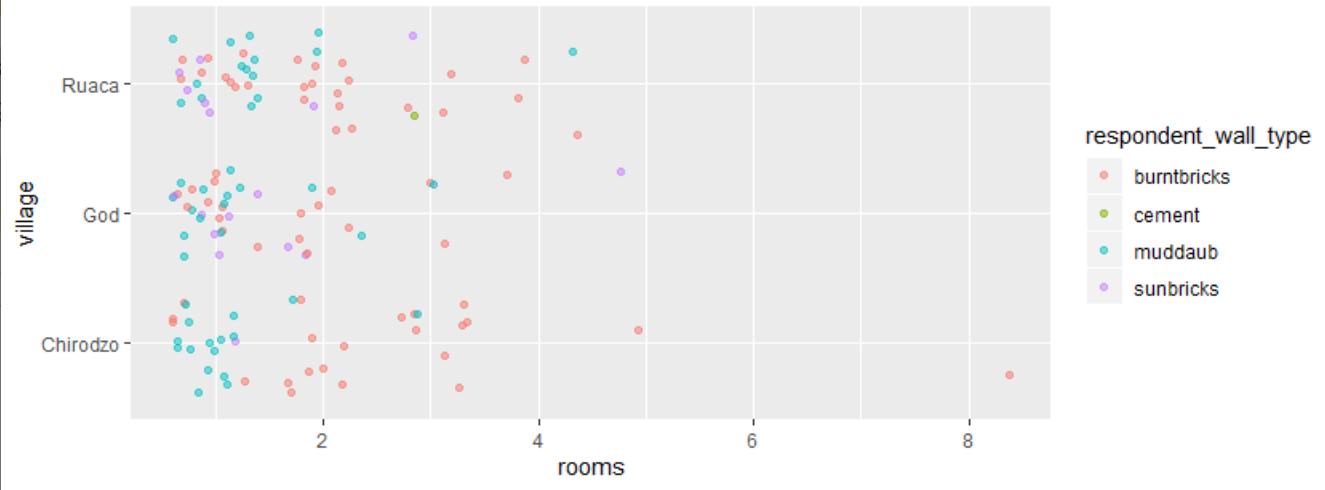
\includegraphics[scale=0.8]{imgdcrcolorplot.PNG}

2. No, there is no way to see trends because the x axis is categorical. A scatterplot is only useful when both axes are numerical. You would be better off with a boxplot.

\end{addmargin}

\textbf{Boxplots}

Use \texttt{geom\_boxplot()} function for boxplots. For example:
\begin{verbatim}
ggplot(data = interviews_plotting, aes(x = respondent_wall_type, y = rooms)) +
    geom_boxplot(alpha = 0) +
    geom_jitter(alpha = 0.5, color = "tomato")    
\end{verbatim}



\newpage
\begin{addmargin}[1cm]{0cm}
\color{gray}
\underline{Exercise:}

Boxplots are useful summaries, but hide the shape of the distribution. For example, if the distribution is bimodal, we would not see it in a boxplot. An alternative to the boxplot is the violin plot, where the shape (of the density of points) is drawn.

1. Replace the box plot with a violin plot; see \texttt{geom\_violin()}.

2. So far, we’ve looked at the distribution of room number within wall type. Try making a new plot to explore the distribution of another variable within wall type.

Create a boxplot for \texttt{liv\_count} for each wall type. Overlay the boxplot layer on a jitter layer to show actual measurements.

3. Add color to the data points on your boxplot according to whether the respondent is a member of an irrigation association \texttt{(memb\_assoc)}.

\color{black}\vspace{0.5em}

1. 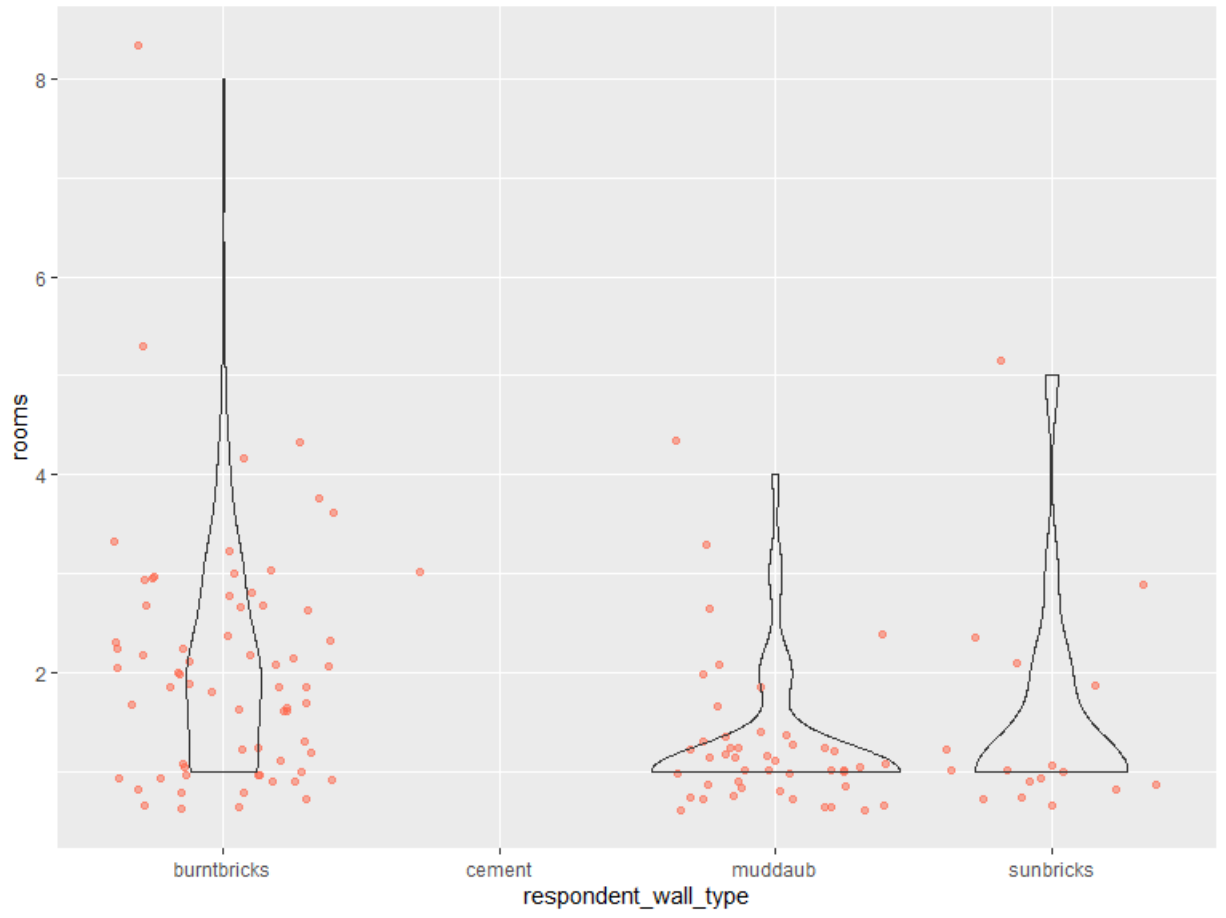
\includegraphics[scale=0.4]{imgdcrviolin.PNG}

2. 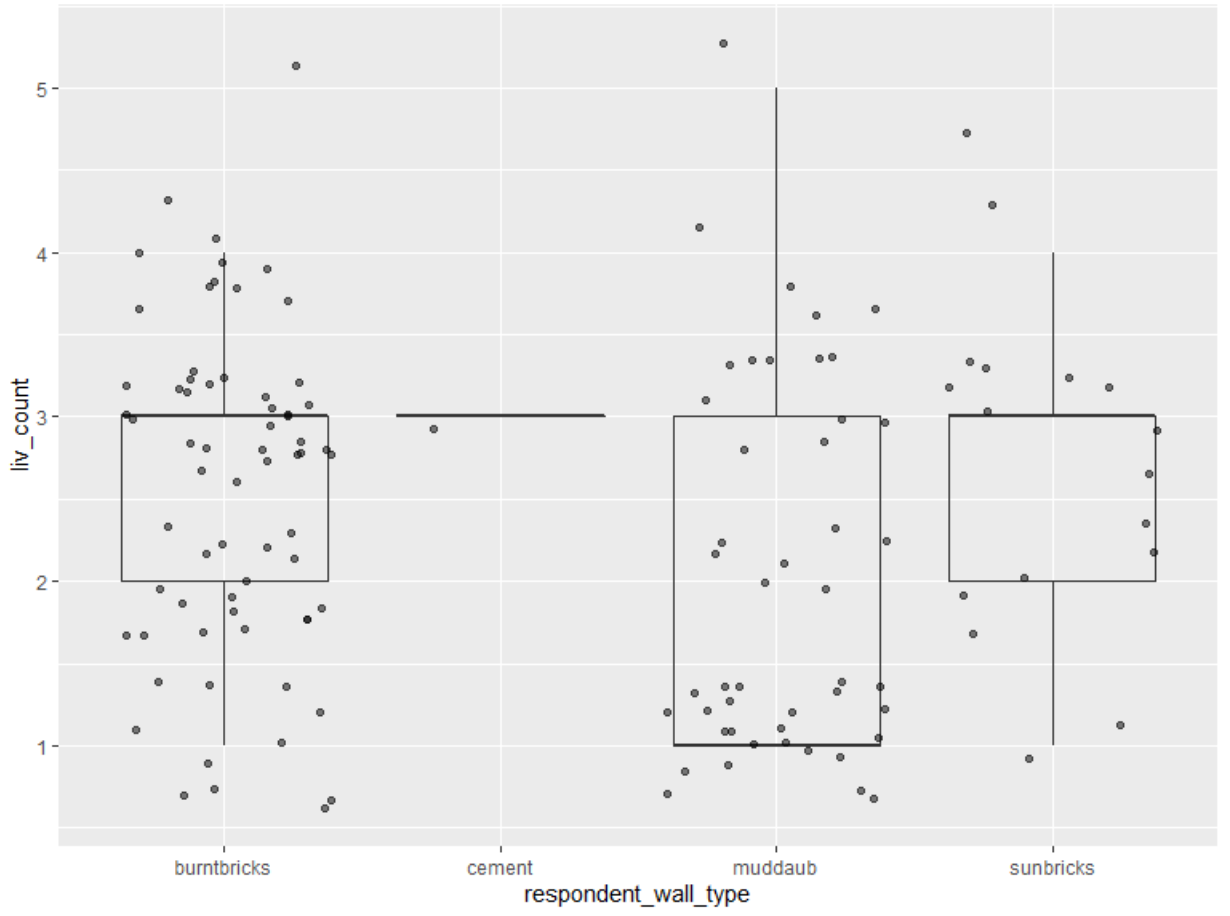
\includegraphics[scale=0.4]{imgdcrboxlivcount.PNG}

3. 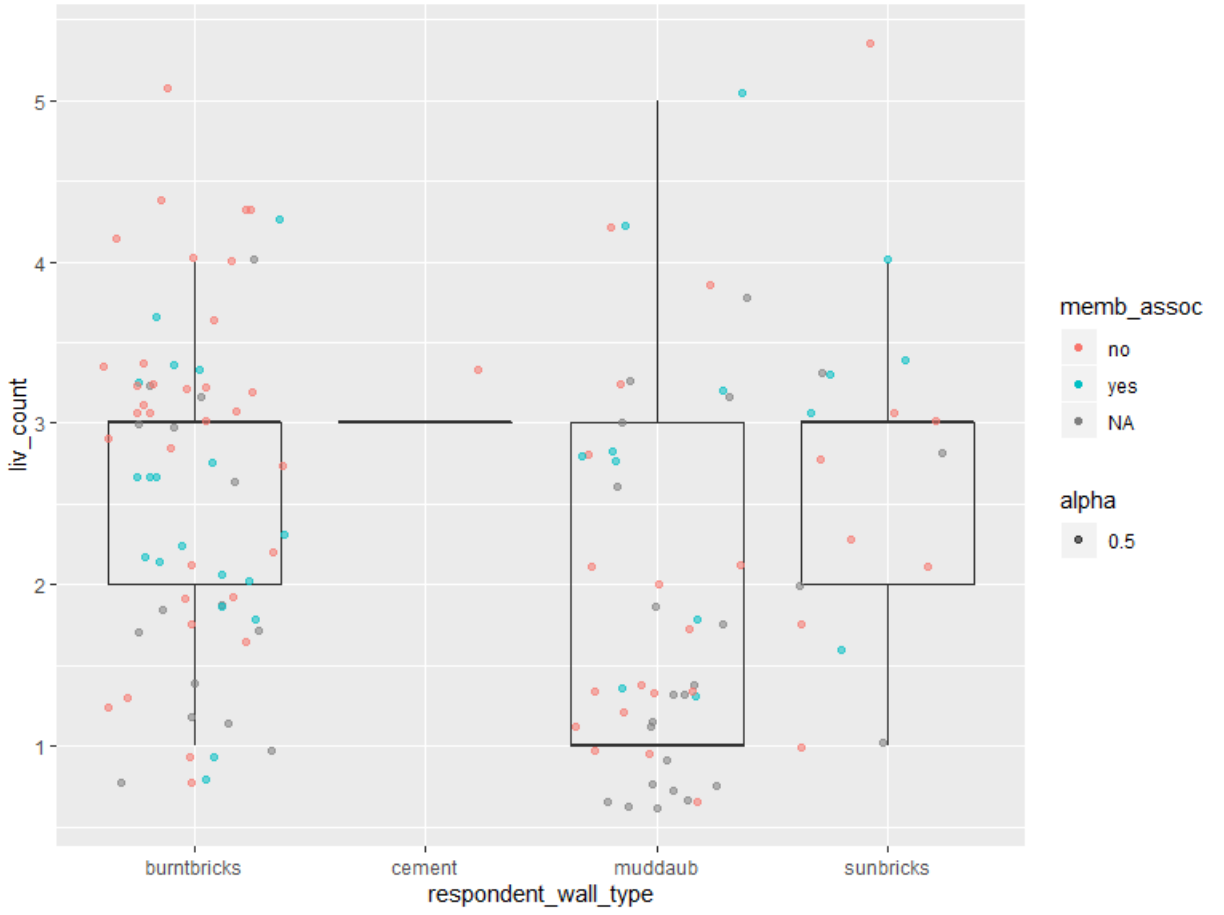
\includegraphics[scale=0.5]{imgdcrboxcolor.PNG}

\end{addmargin}

\newpage\textbf{Barplots}

Use \texttt{geom\_bar()} with any variable for x, and y will by default act as count. Use \texttt{(fill=village)} to colour sections of the barplot by village.

To compare proportionally, create a new data frame with your calculated percentages. For example:
\begin{verbatim}
percent_wall_type <- interviews_plotting %>%
    filter(respondent_wall_type != "cement") %>%
    count(village, respondent_wall_type) %>%
    group_by(village) %>%
    mutate(percent = n / sum(n)) %>%
    ungroup()
    
 ggplot(percent_wall_type, aes(x=village, y=percent, fill=respondent_wall_type)) +
     geom_bar(stat = "identity", position = "dodge")
\end{verbatim}
In the above example we removed "cement", since there was only one data entry.

\vspace{0.5em}
\begin{addmargin}[1cm]{0cm}
\color{gray}
\underline{Exercise:}

Create a bar plot showing the proportion of respondents in each village who are or are not part of an irrigation association (memb\_assoc). Include only respondents who answered that question in the calculations and plot. Which village had the lowest proportion of respondents in an irrigation association?

\color{black}\vspace{0.5em}

\begin{verbatim}
percent_memb_assoc <- interviews_plotting %>%
    filter(!is.na(memb_assoc) %>%
    count(village, memb_assoc) %>%
    group_by(village) %>%
    mutate(percent = n / sum(n)) %>%
    ungroup()
    
ggplot(percent_memb_assoc, aes(x=village,y=percent,fill=memb_assoc)) +
    geom_bar(stat = "identity", position = "dodge")
\end{verbatim}
The bar plot shows Ruaca has the lowest proportion of membership with an irrigation association.
\end{addmargin}

\vspace{0.5em}\textbf{Labels and Faceting}

You may need the axes to be labelled differently from how they appear in your data. You may want to wrap them into sections, such as this example with a separate graph per village. For readability, you might want to make it B+W friendly for an article.
\begin{verbatim}
ggplot(percent_wall_type, aes(x=village, y=percent, fill=respondent_wall_type)) +
    geom_bar(stat = "identity", position = "dodge") +
    labs(title="Proportion of wall type by village",
         x="Wall Type",
         y="Percent") +
    facet_wrap(~ village)
    theme_bw() +
    theme(panel.grid = element_blank())
\end{verbatim}

\newpage\textbf{Themes}

Cheat sheet for making graphs look good can be found \href{https://rstudio.com/wp-content/uploads/2016/11/ggplot2-cheatsheet-2.1.pdf}{here}. If you like the theme you made, you can save it to a variable as a preset:
\begin{verbatim}
grey_theme <- theme(axis.text.x=element_text(colour="grey20",size=12,angle=45,
    hjust=0.5,vjust=0.5),
                    axis.text.y = element_text(colour = "grey20", size = 12),
                    text = element_text(size = 16),
                    plot.title = element_text(hjust = 0.5))


ggplot(percent_items, aes(x = village, y = percent)) +
    geom_bar(stat = "identity", position = "dodge") +
    facet_wrap(~ items) +
    labs(title = "Percent of respondents in each village \n who owned each item",
         x = "Village",
         y = "Percent of Respondents") +
    grey_theme    
\end{verbatim}

\textbf{Exporting}

You can export the finished plot to your chosen format. Don't use the Export tab in the Plot pan, it will be too low res. Use \texttt{ggsave()}, so you can change arguments \texttt{(width, height, dpi)}
\begin{verbatim}
my_plot <- ggplot(percent_items, aes(x = village, y = percent)) +
    geom_bar(stat = "identity", position = "dodge") +
    facet_wrap(~ items) +
    labs(title = "Percent of respondents in each village \n who owned each item",
         x = "Village",
         y = "Percent of Respondents") +
    theme_bw() +
    theme(axis.text.x = element_text(colour = "grey20", size = 12, angle = 45, 
    hjust = 0.5, vjust = 0.5),
          axis.text.y = element_text(colour = "grey20", size = 12),
          text = element_text(size = 16),
          plot.title = element_text(hjust = 0.5))

ggsave("fig_output/name_of_file.png", my_plot, width = 15, height = 10)    
\end{verbatim}

(For above example make sure you have a folder called fig\_output in your cwd.)

\newpage\section{08.03.20 - Proof of Concept: PICO Presentation}

A Presentation of Interactive COntent (\href{https://egu2019.eu/PICO_how-to_guide_to_PICO.pdf}{PICO}) is a style of presentation where you "hook" an audience in with two minutes of speech time, and the rest of the information can be found on an interactive screen with the rest of your slides. 

\textbf{Creating a lightning talk}

The angle I should go with is how this can improve the efficiency of writing for researchers. Looking at videos and other examples, I'm getting a picture that the speech should feel more like a sales pitch or a youtube edutainment video, rather than a formal speech towards scientists. I think it's a good idea, because with so many researchers studying so many interesting ideas that I don't have the background to appreciate, this means stuff that's relevant to me from other disciplines is easier to spot.

\textbf{First two slides}

For the two-minute madness speech, I can explain what the PoC is and what it does. I start with solving a problem: Feeling overwhelmed by 20 000 words target of the Masters thesis. I describe how I chunk this unmanageable task into sections, and those sections into subsections. I show how the frame works, and what benefit it has.

\textbf{Non-presentation slides}

This is where it gets tricky: there's not a lot more to the frame than the introduction. Things I can add for further convincing:

\begin{itemize}
    \item Drawbacks of the current alternative
    \item Benefits of chunking
    \item Writing efficiency techniques
    
\end{itemize}


%"Intentions, Actions, Results"

\newpage\section{Library of LaTeX Errors}
\begin{itemize}
\renewcommand{\labelitemi}{}
    \item \ref{error:er1} Rich Text Mode 
    \item \ref{error:er2} Bullet List 
    \item \ref{error:er3} Using Packages
    \item \ref{error:er4} Right Alignment
    \item \ref{error:er5} Document Style
    \item \ref{error:er6} Paragraph Spacing
    \item \ref{error:er7} Special Characters
    \item \ref{error:er8} Image Insertion
    \item \ref{error:er9} Margins
    \item \ref{error:er10} Automatic Dating
    \item \ref{error:er11} Displaying Japanese Characters
    \item \ref{error:er14} Undefined Control Sequence
    \item \ref{error:er15} Hyperref Token Not Allowed
\end{itemize}


\section{Library of Data Carpentry Errors}
\begin{itemize}
\renewcommand{\labelitemi}{}
    \item \ref{error:er12} GUI/CLI Confusion
    \item \ref{error:er13} Shell: Command Not Found
    \item \ref{error:er16} Shell: Does Not Print Or Loop
    \item \ref{error:er17} Shell: Pipe Functionality
    \item \ref{error:er18} Shell: Grepping Singular Words
    \item \ref{error:er19} R: Multiple Functions
    \item \ref{error:er20} R: Renaming and Reordering Factors
\end{itemize}

\end{document}





% commit details: what was added, deleted, changed, AND how it went

% CODESUBSECTIONCODE
\subsection{\href{http://www.abc.com}{\textbf{Page Title}}}
\color{gray}
\underline{Questions}



\underline{Objectives}



\color{black}
\vspace{1em}



\vspace{0.5em}
\begin{addmargin}[1cm]{0cm}
\color{gray}
\underline{Exercise:}

1. 
\\2. 

\color{black}\vspace{0.5em}

1.
\\2.

\end{addmargin}